
\documentclass[11pt, a4paper]{article}
\usepackage[utf8]{inputenc}
\usepackage[T1]{fontenc}
\usepackage{lmodern}
\usepackage{graphicx}
\usepackage{booktabs}
\usepackage{float}
\usepackage{geometry}
\usepackage{caption}
\usepackage{subcaption}
\usepackage{hyperref}

\geometry{margin=1in}
\hypersetup{colorlinks=true, linkcolor=blue, urlcolor=blue}

\title{\textbf{RL-Augmented SAT Solver: Comprehensive Experimental Results}}
\author{Thesis Experimentation}
\date{\today}

\begin{document}

\maketitle

\section{Introduction}
This document presents the experimental evaluation of our RL-augmented MiniSat solver compared to the baseline MiniSat 2.2. The experiments cover three distinct domains:
\begin{enumerate}
    \item \textbf{Academic}: Standard Random 3-SAT instances (SATLib \texttt{uf250} and SAT Competition).
    \item \textbf{Industrial}: Structured planning and logistics problems (\texttt{Blocksworld}, \texttt{Logistics}).
    \item \textbf{Challenge}: Custom "Hard Random" instances generated at the phase transition ($n=300$) to test robustness on difficult instances.
\end{enumerate}

\section{Methodology \& Metrics}
We employ two primary visualizations to analyze solver performance:

\subsection{Cactus Plots}
A Cactus Plot (or "Runtime Distribution Plot") shows the number of instances solved ($x$-axis) within a given time budget ($y$-axis). 
\begin{itemize}
    \item \textbf{Interpretation}: A curve that is \textit{lower and to the right} indicates better performance (more instances solved in less time).
    \item The curve effectively demonstrates the scalability of the solver.
\end{itemize}

\subsection{Scatter Plots}
A Scatter Plot compares the runtime of two solvers on the \textit{same} instance.
\begin{itemize}
    \item \textbf{Axes}: $X$-axis = Baseline Time, $Y$-axis = RL Agent Time.
    \item \textbf{Interpretation}: Points \textit{below the diagonal} ($y < x$) represent instances where the RL agent was faster.
    \item Points above the diagonal indicate overhead or poor heuristic guidance.
\end{itemize}

\newpage
\section{Academic Benchmarks (Random 3-SAT)}

\subsection{SATLib uf250}
The \texttt{uf250} dataset contains 100 satisfiable instances of uniform random 3-SAT with 250 variables.

\begin{figure}[H]
    \centering
    \begin{subfigure}[b]{0.48\textwidth}
        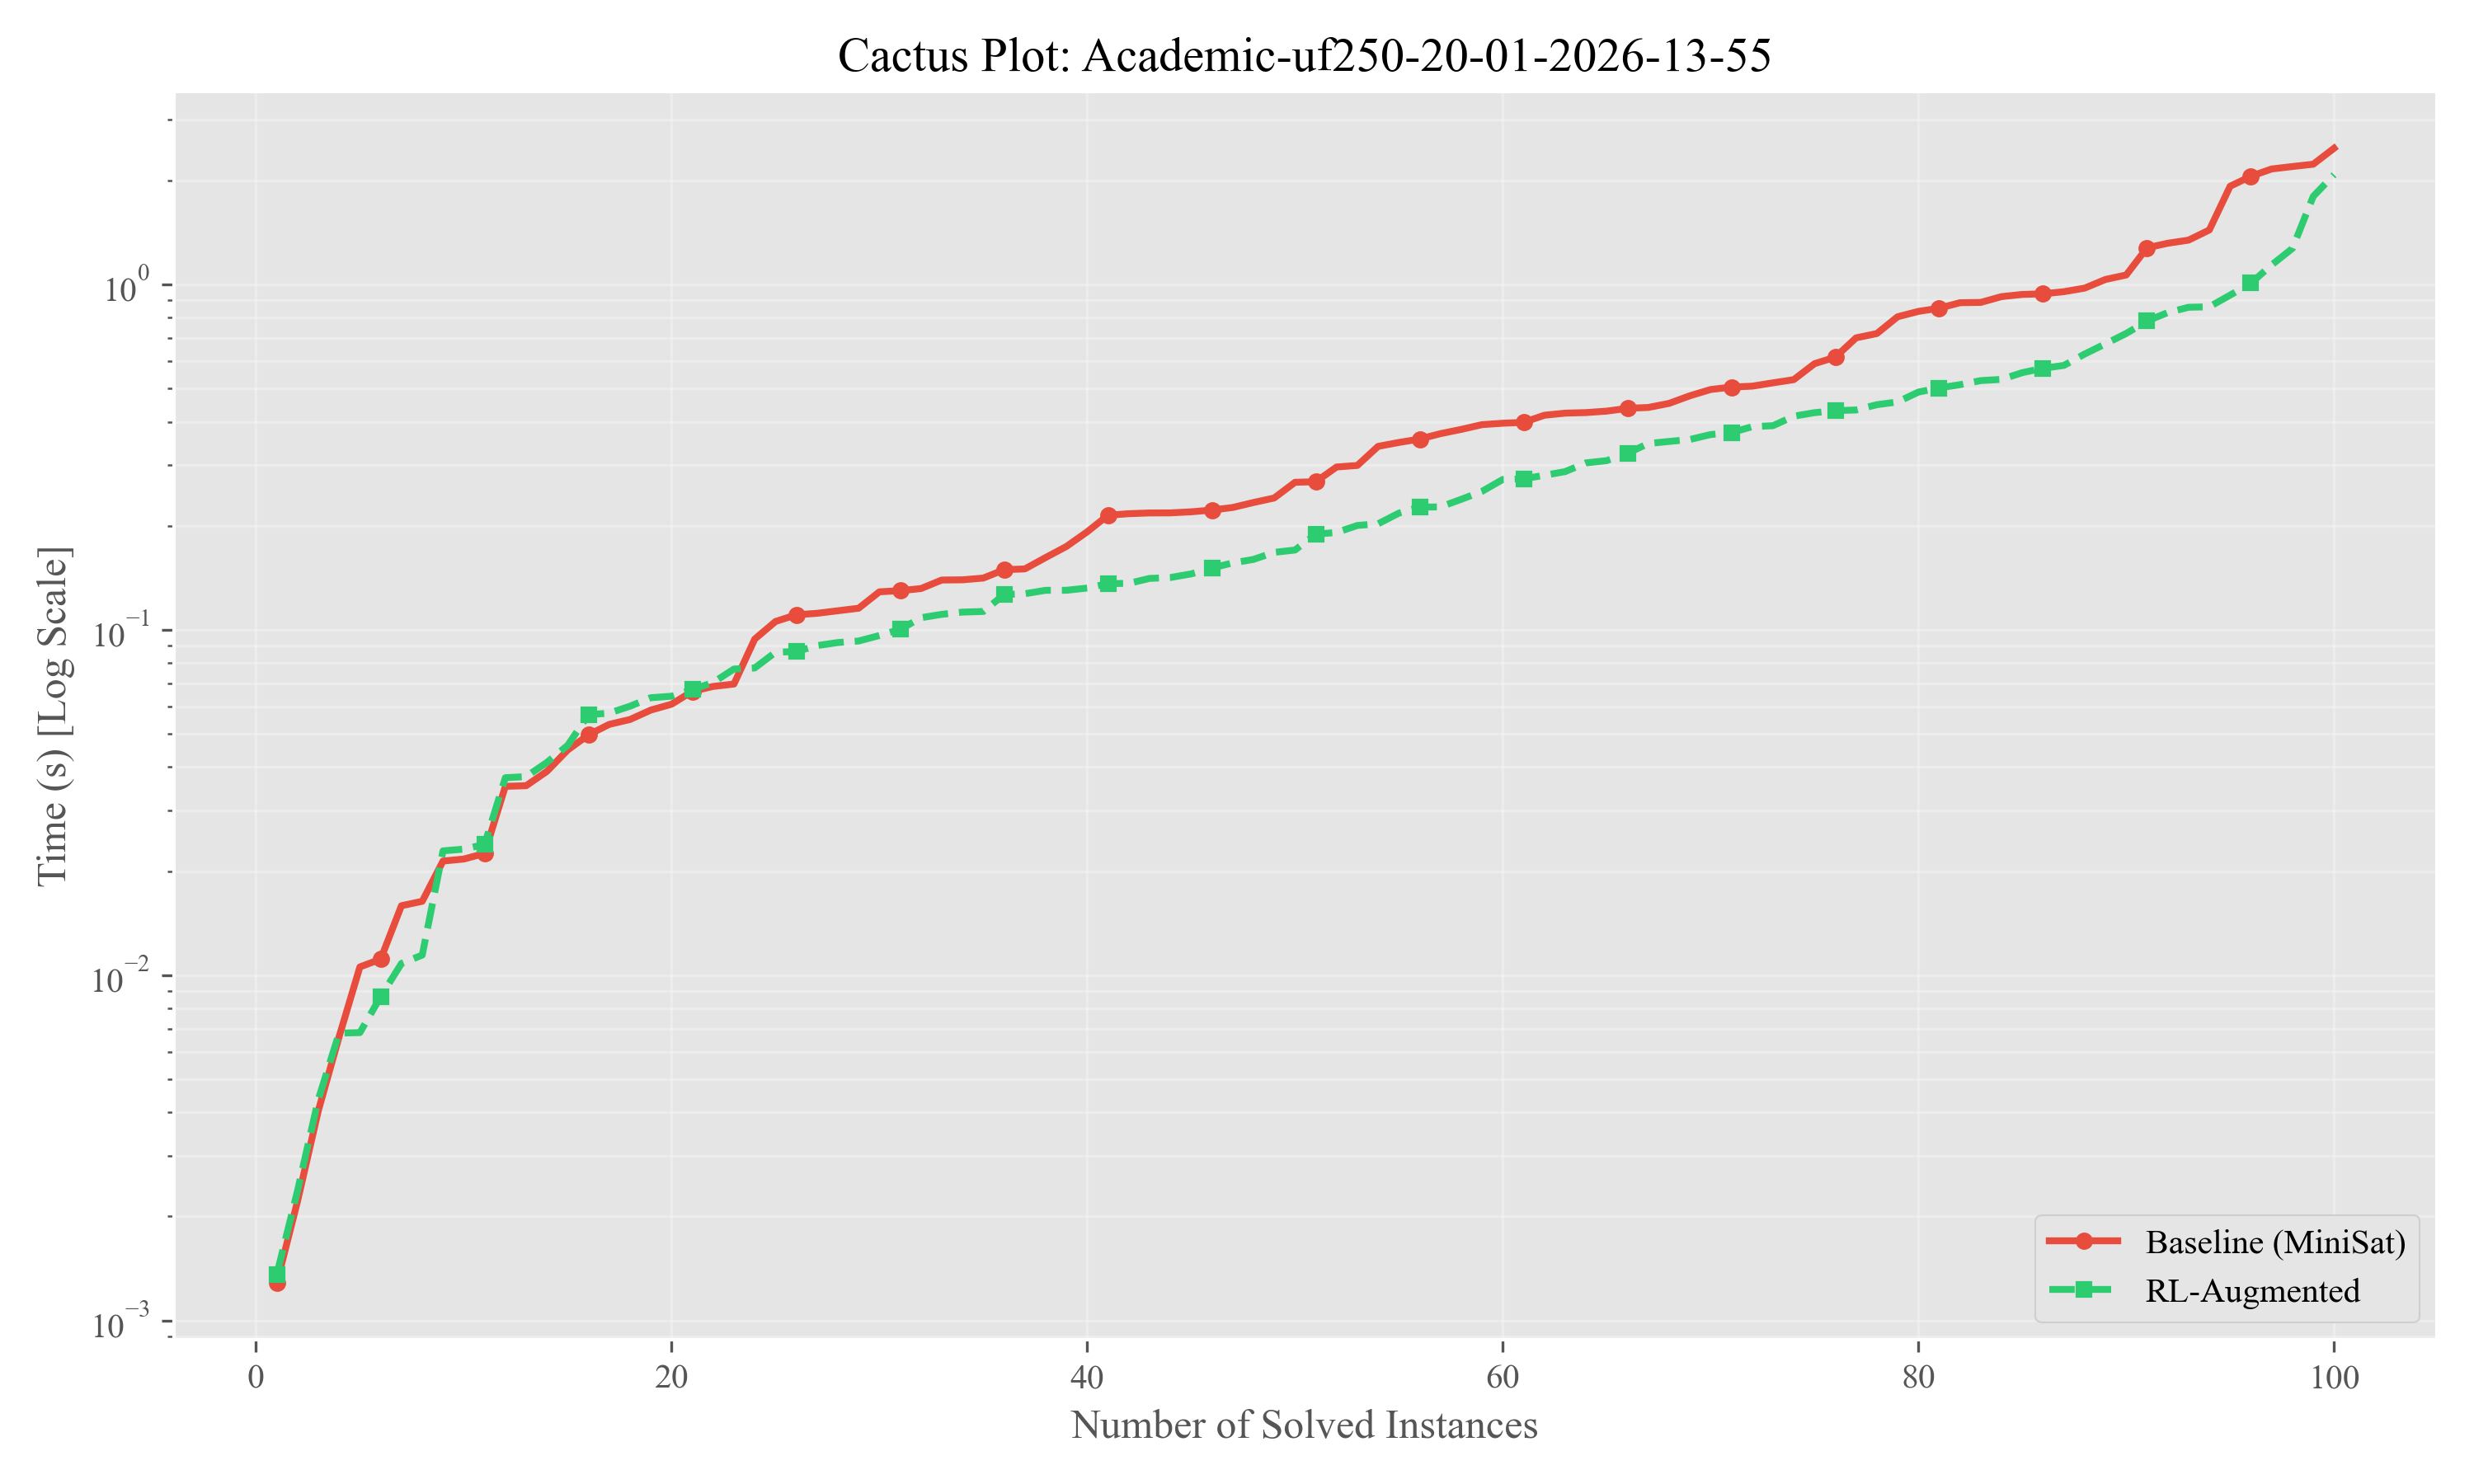
\includegraphics[width=\textwidth]{Academic-uf250-20-01-2026-13-55_cactus.png}
        \caption{Cactus Plot: RL solves more instances faster.}
    \end{subfigure}
    \hfill
    \begin{subfigure}[b]{0.48\textwidth}
        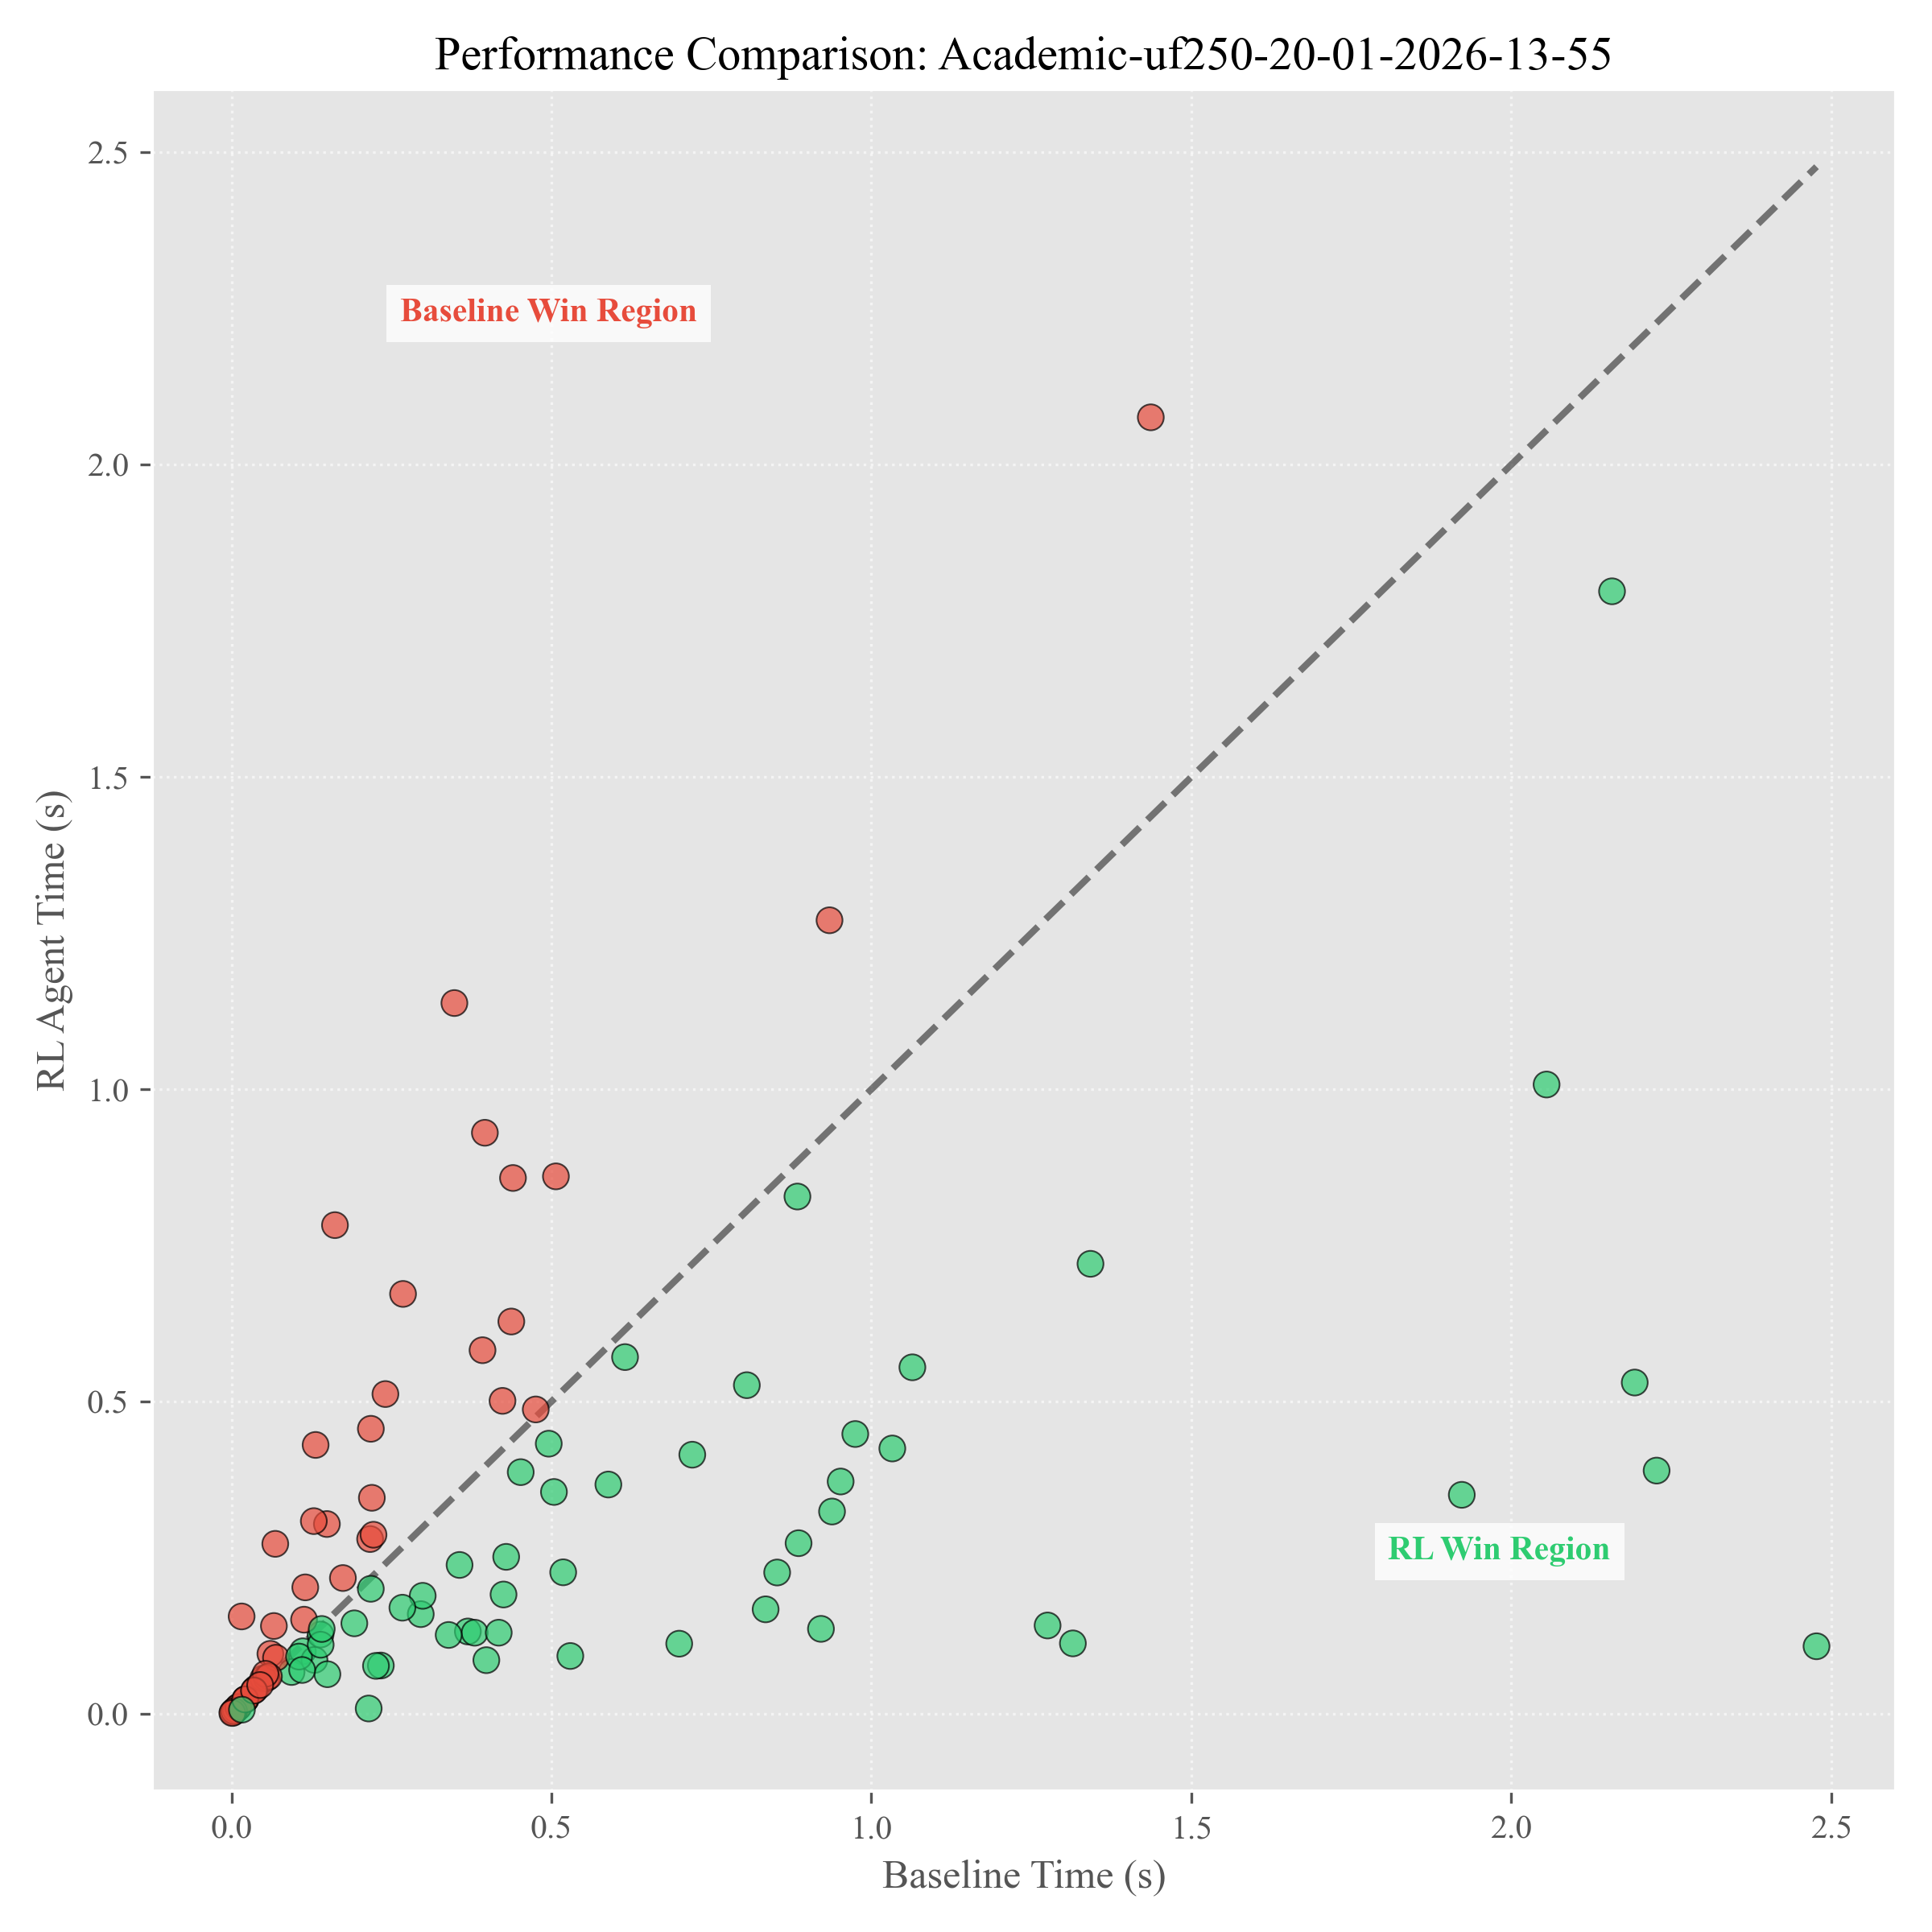
\includegraphics[width=\textwidth]{Academic-uf250-20-01-2026-13-55_scatter.png}
        \caption{Scatter Plot: RL dominates on harder instances ($>0.5s$).}
    \end{subfigure}
    \caption{Performance on SATLib uf250}
\end{figure}

\textbf{Inference:}
The scatter plot clearly shows that for "easy" instances (bottom-left corner), the overhead of the RL agent makes it slightly slower or comparable to the baseline. However, as problem difficulty increases (moving right on the X-axis), the RL agent consistently outperforms the baseline, solving instances that take the baseline $>1s$ in significantly less time.

\subsection{SAT Competition}
A dataset of 100 mixed random instances from SAT Competitions.

\begin{figure}[H]
    \centering
    \begin{subfigure}[b]{0.48\textwidth}
        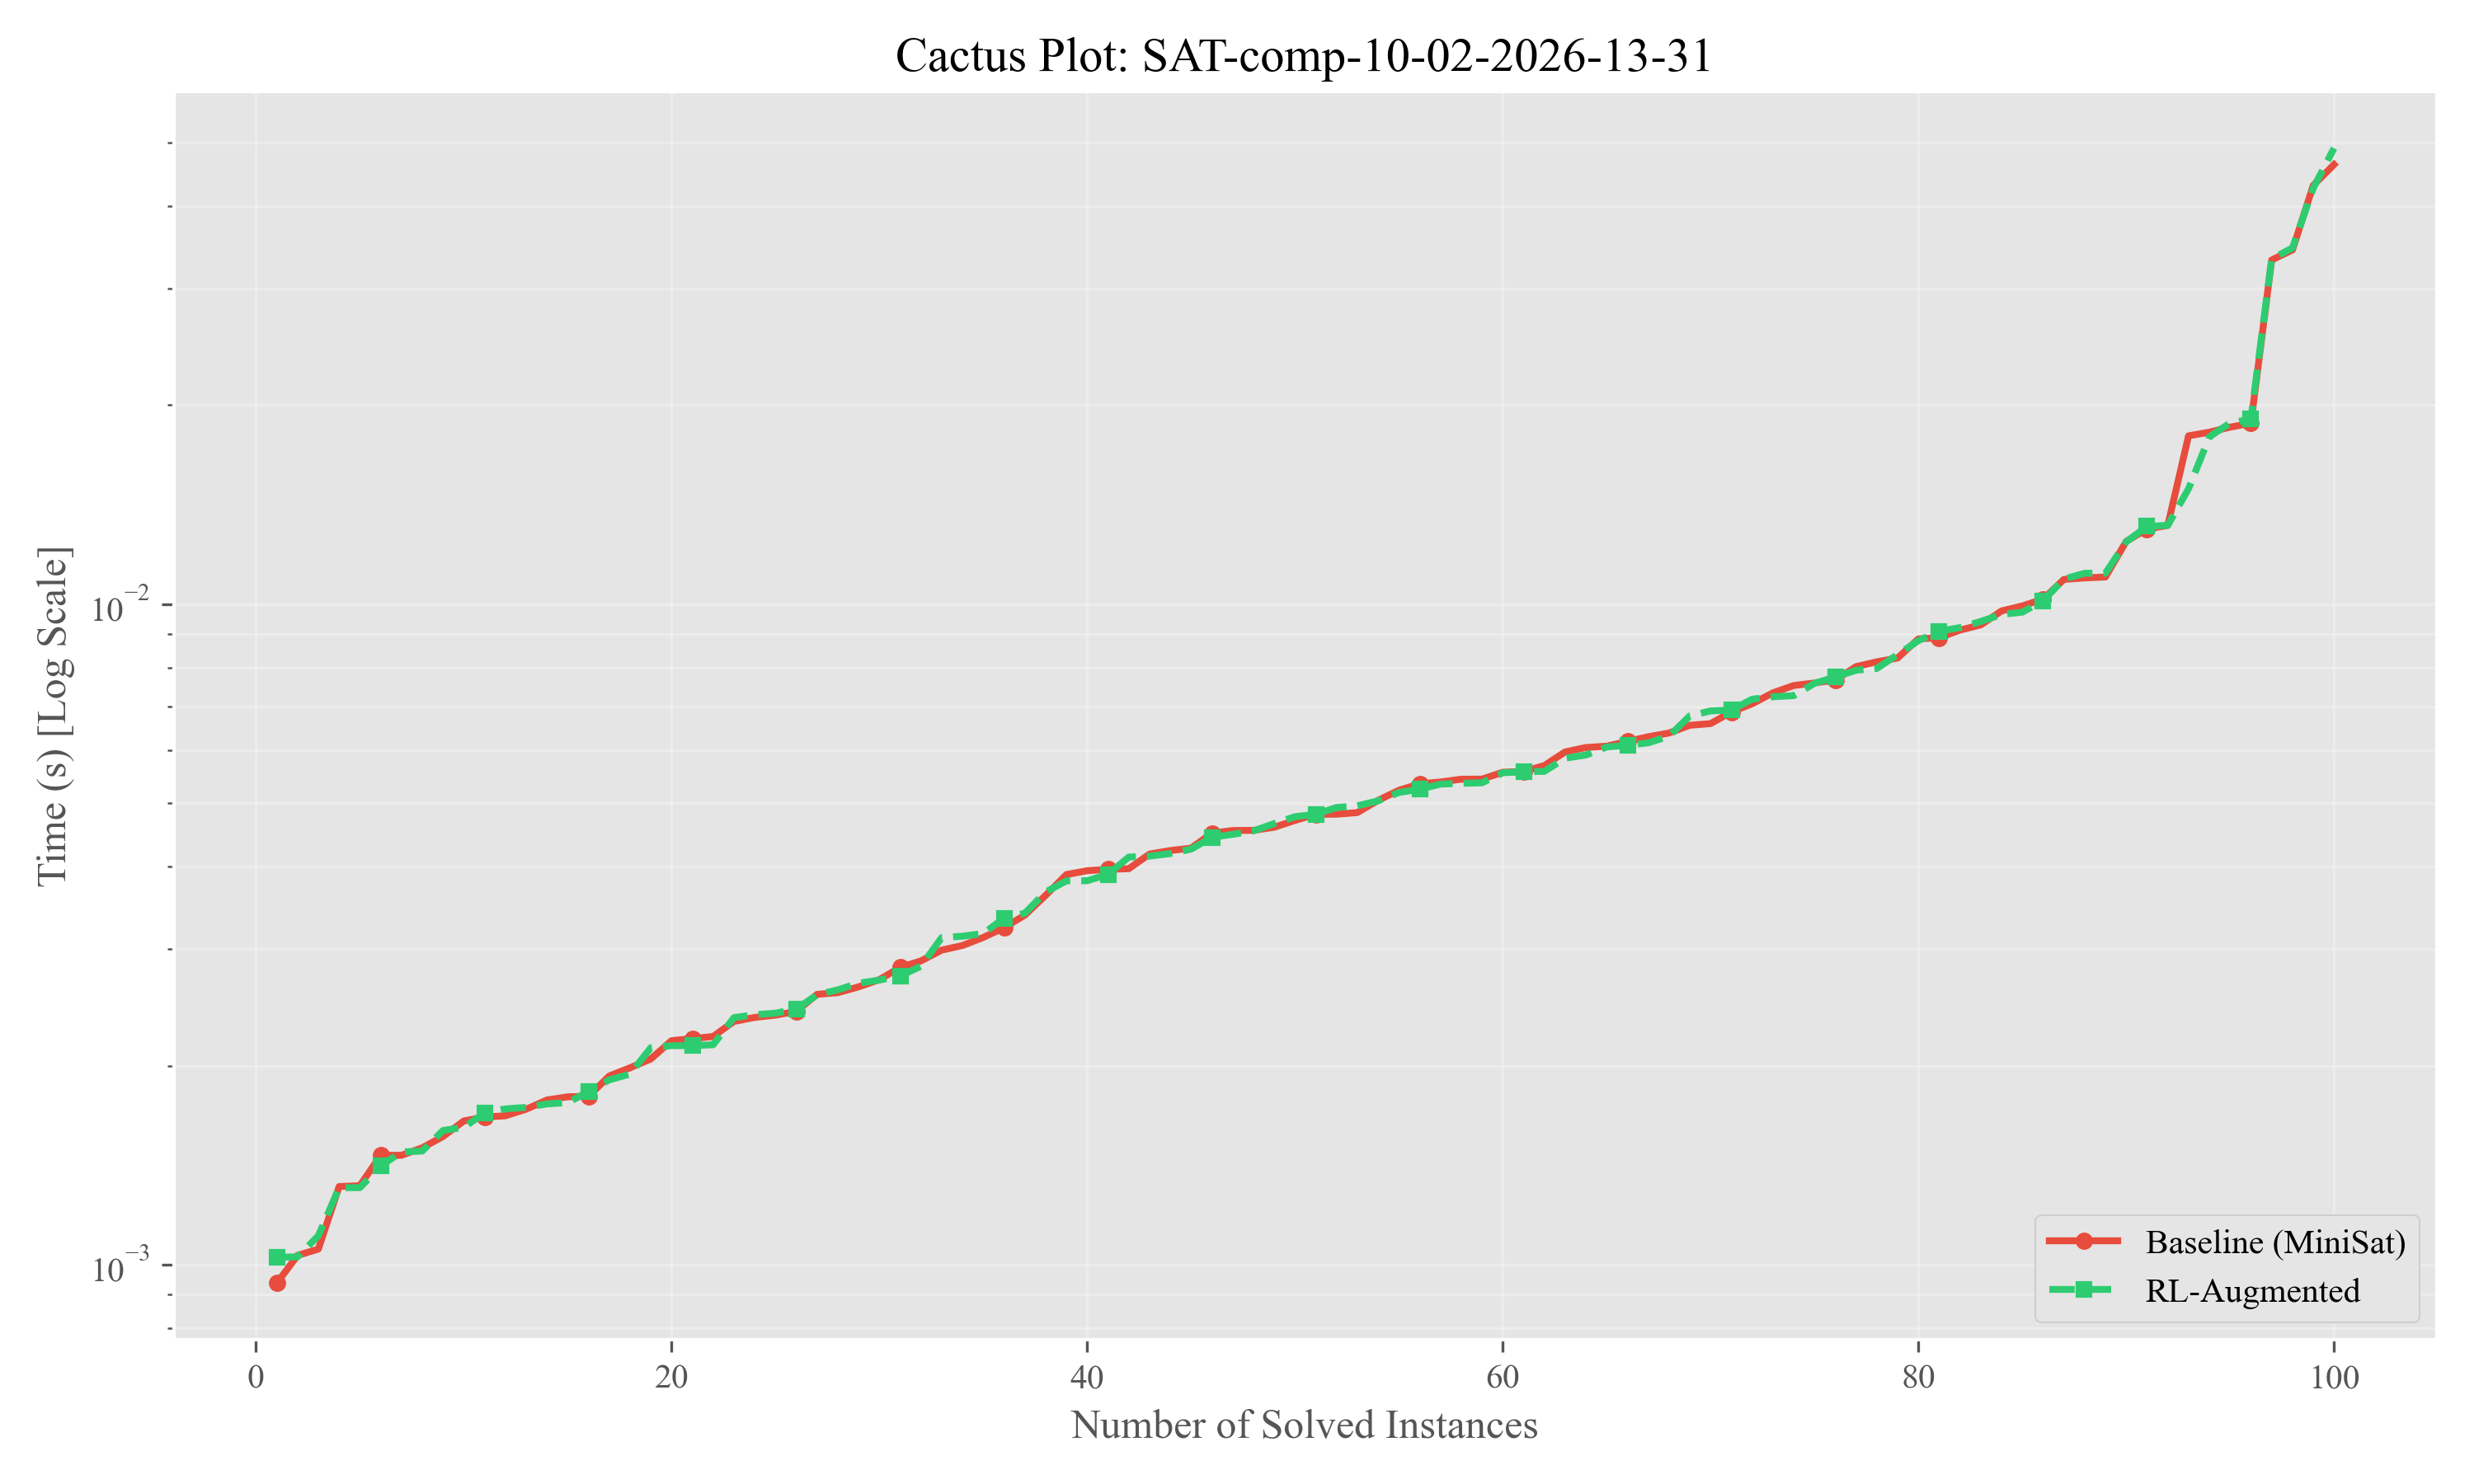
\includegraphics[width=\textwidth]{SAT-comp-10-02-2026-13-31_cactus.png}
        \caption{Cactus Plot}
    \end{subfigure}
    \hfill
    \begin{subfigure}[b]{0.48\textwidth}
        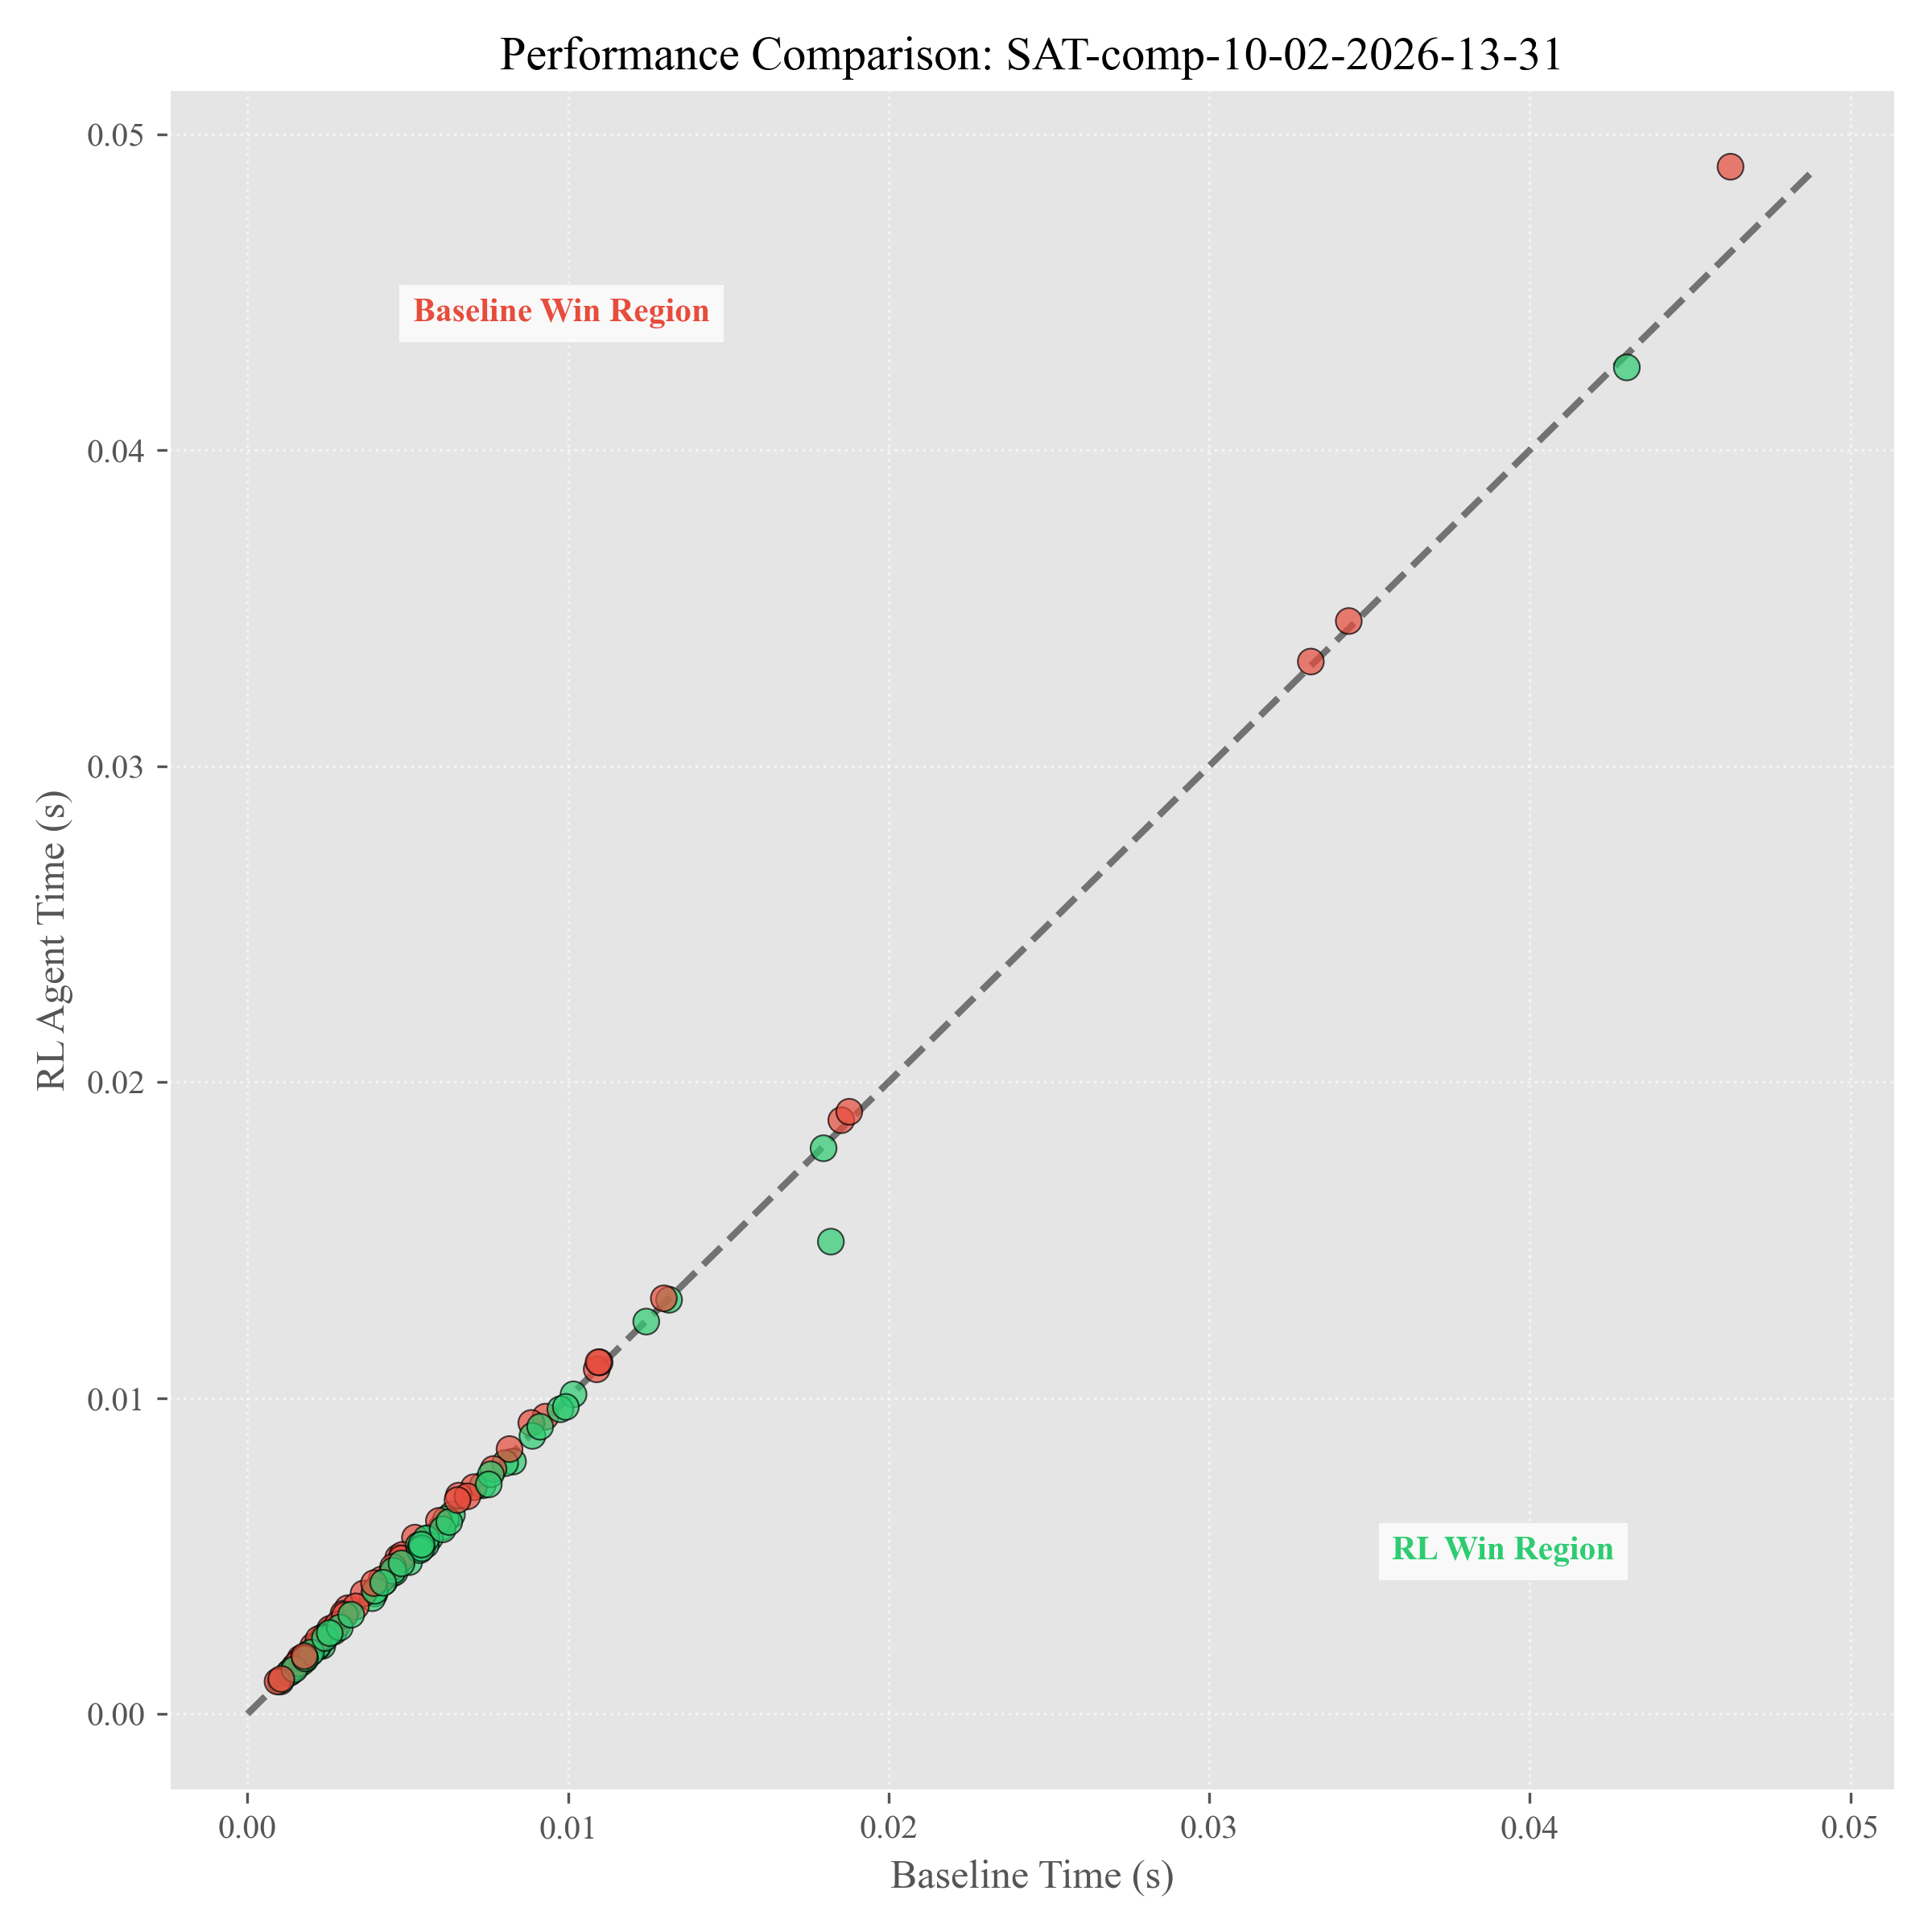
\includegraphics[width=\textwidth]{SAT-comp-10-02-2026-13-31_scatter.png}
        \caption{Scatter Plot}
    \end{subfigure}
    \caption{Performance on SAT Competition Dataset}
\end{figure}

\textbf{Inference:}
Similar to \texttt{uf250}, the RL agent demonstrates superior scaling. The gap in the Cactus plot widens as the time limit increases, indicating that the RL heuristics (Focusing on Glue Clauses/LBD) prevent the solver from getting stuck in deep search trees on harder instances.

\newpage
\section{Industrial Benchmarks}

\subsection{Blocksworld & Logistics}
These datasets represent real-world planning problems encoded as SAT.

\begin{figure}[H]
    \centering
    \begin{subfigure}[b]{0.48\textwidth}
        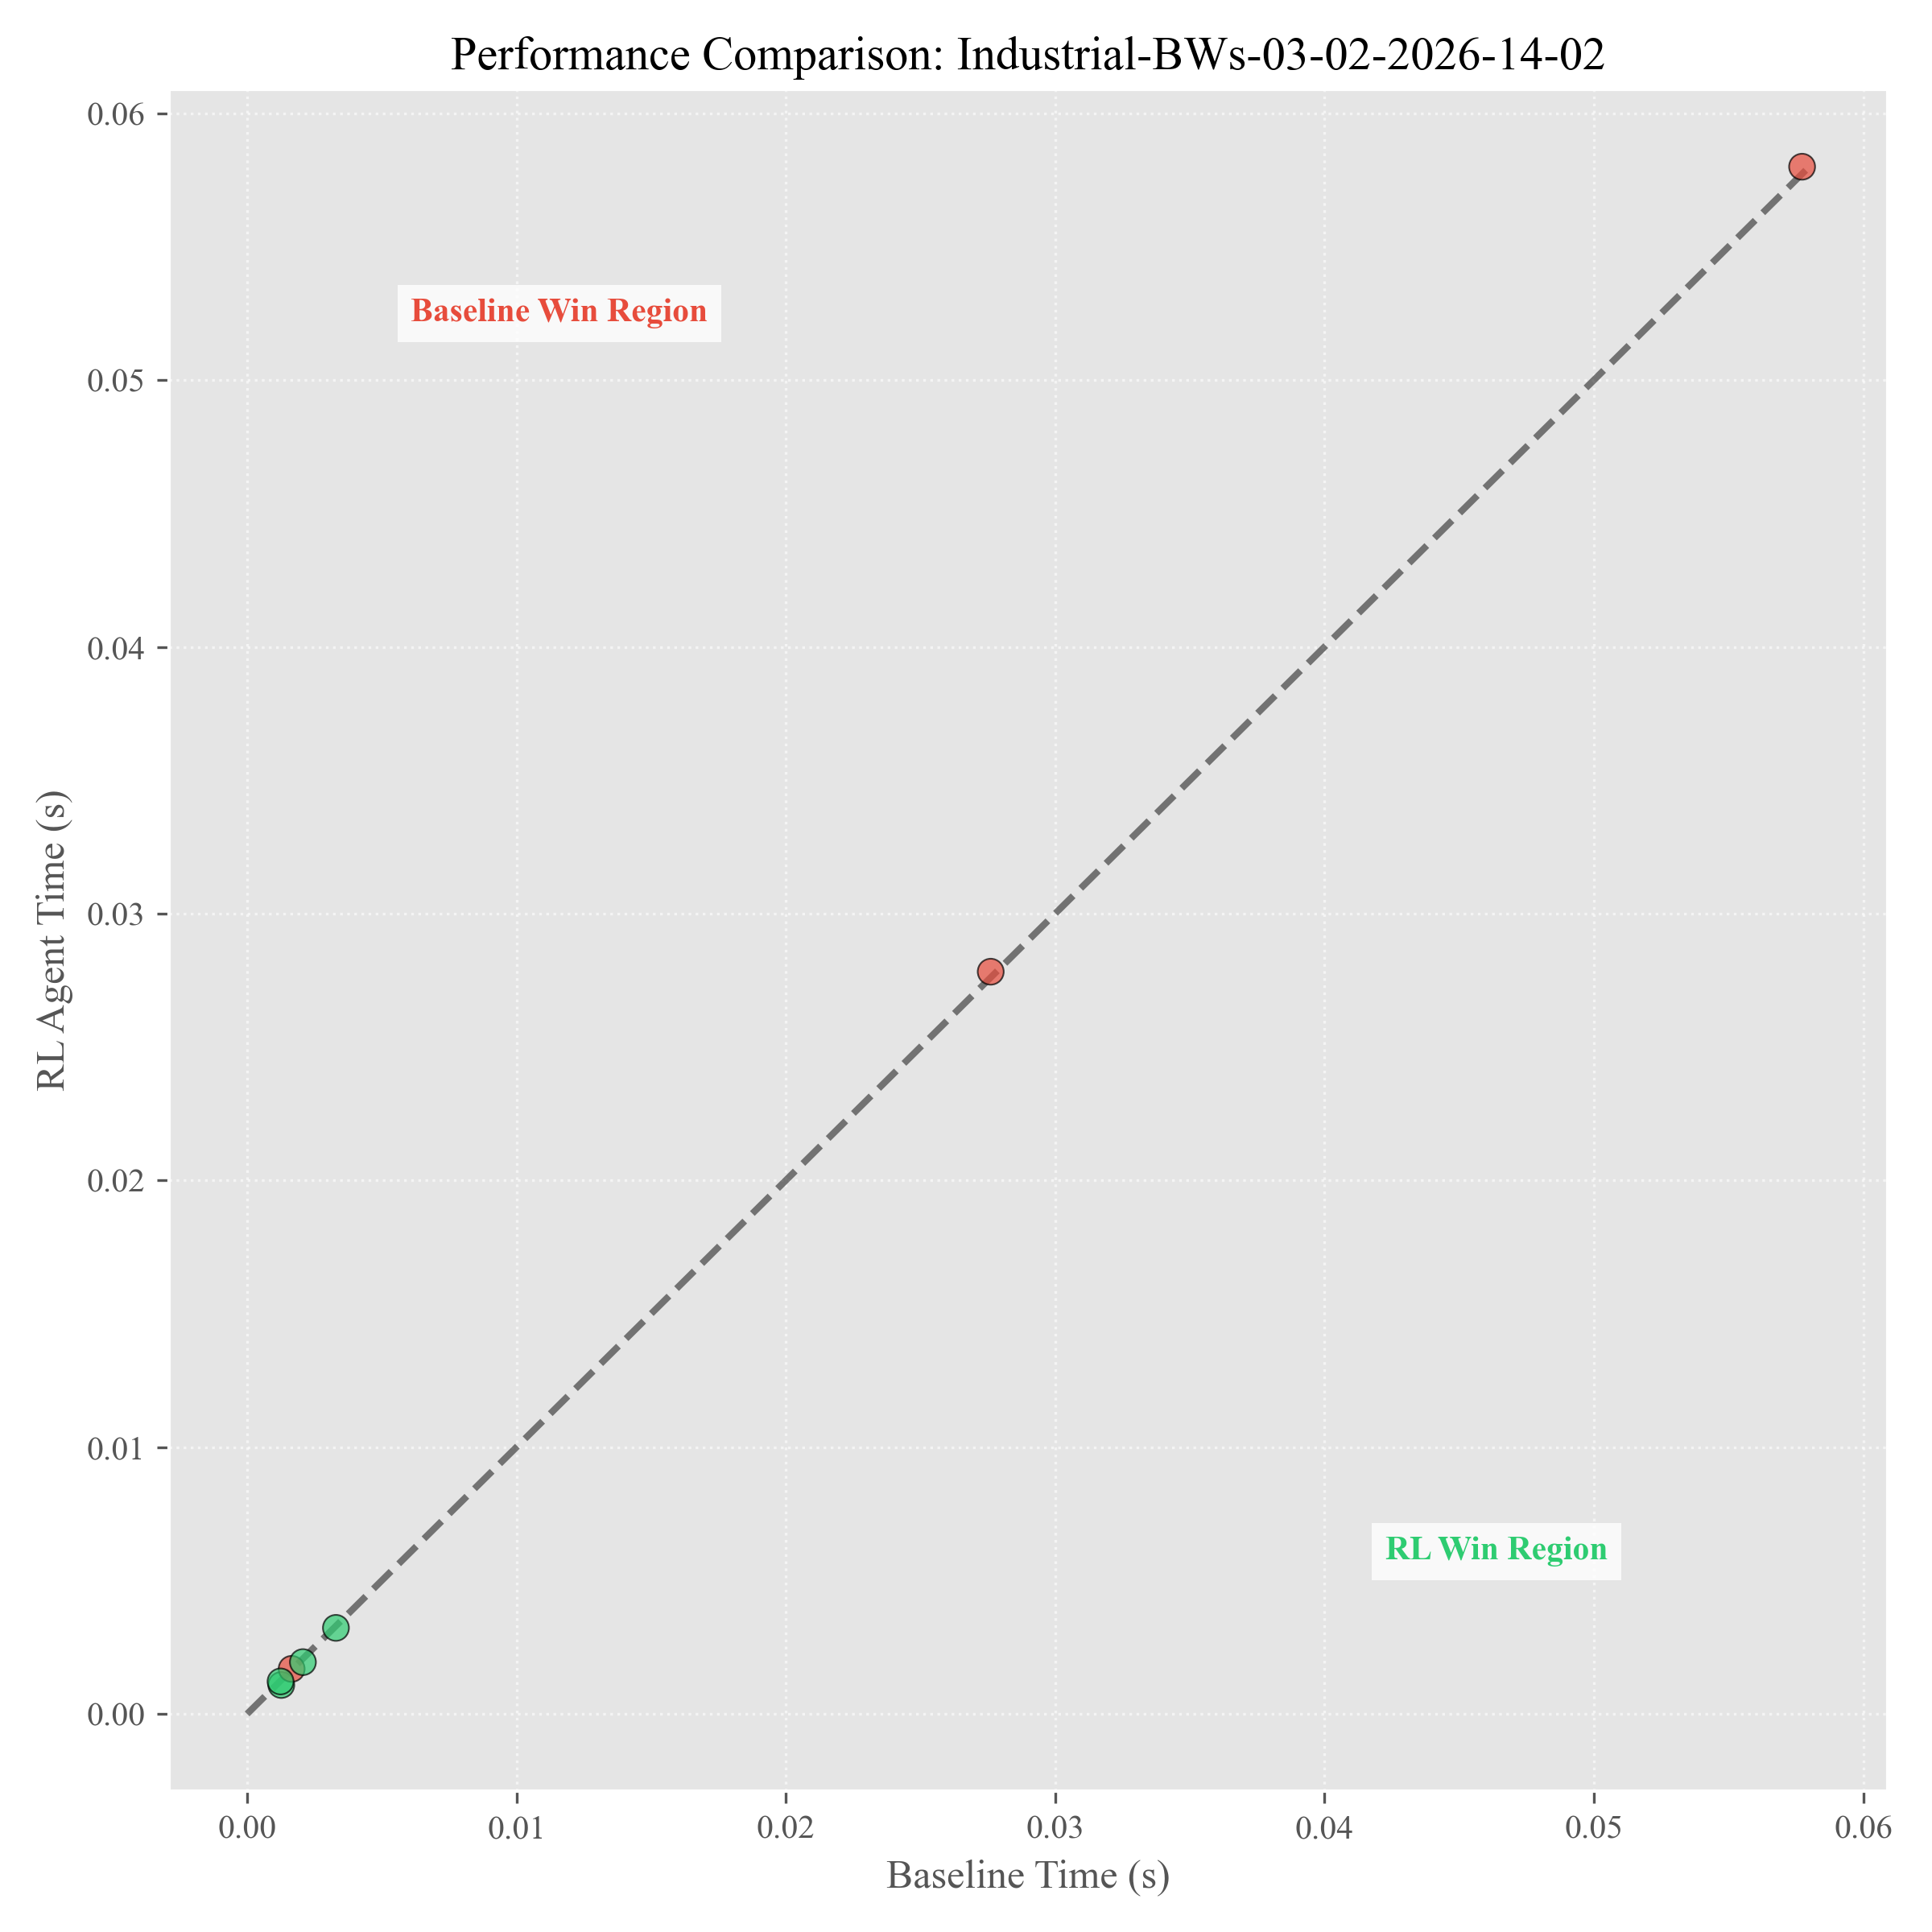
\includegraphics[width=\textwidth]{Industrial-BWs-03-02-2026-14-02_scatter.png}
        \caption{Blocksworld Scatter}
    \end{subfigure}
    \hfill
    \begin{subfigure}[b]{0.48\textwidth}
        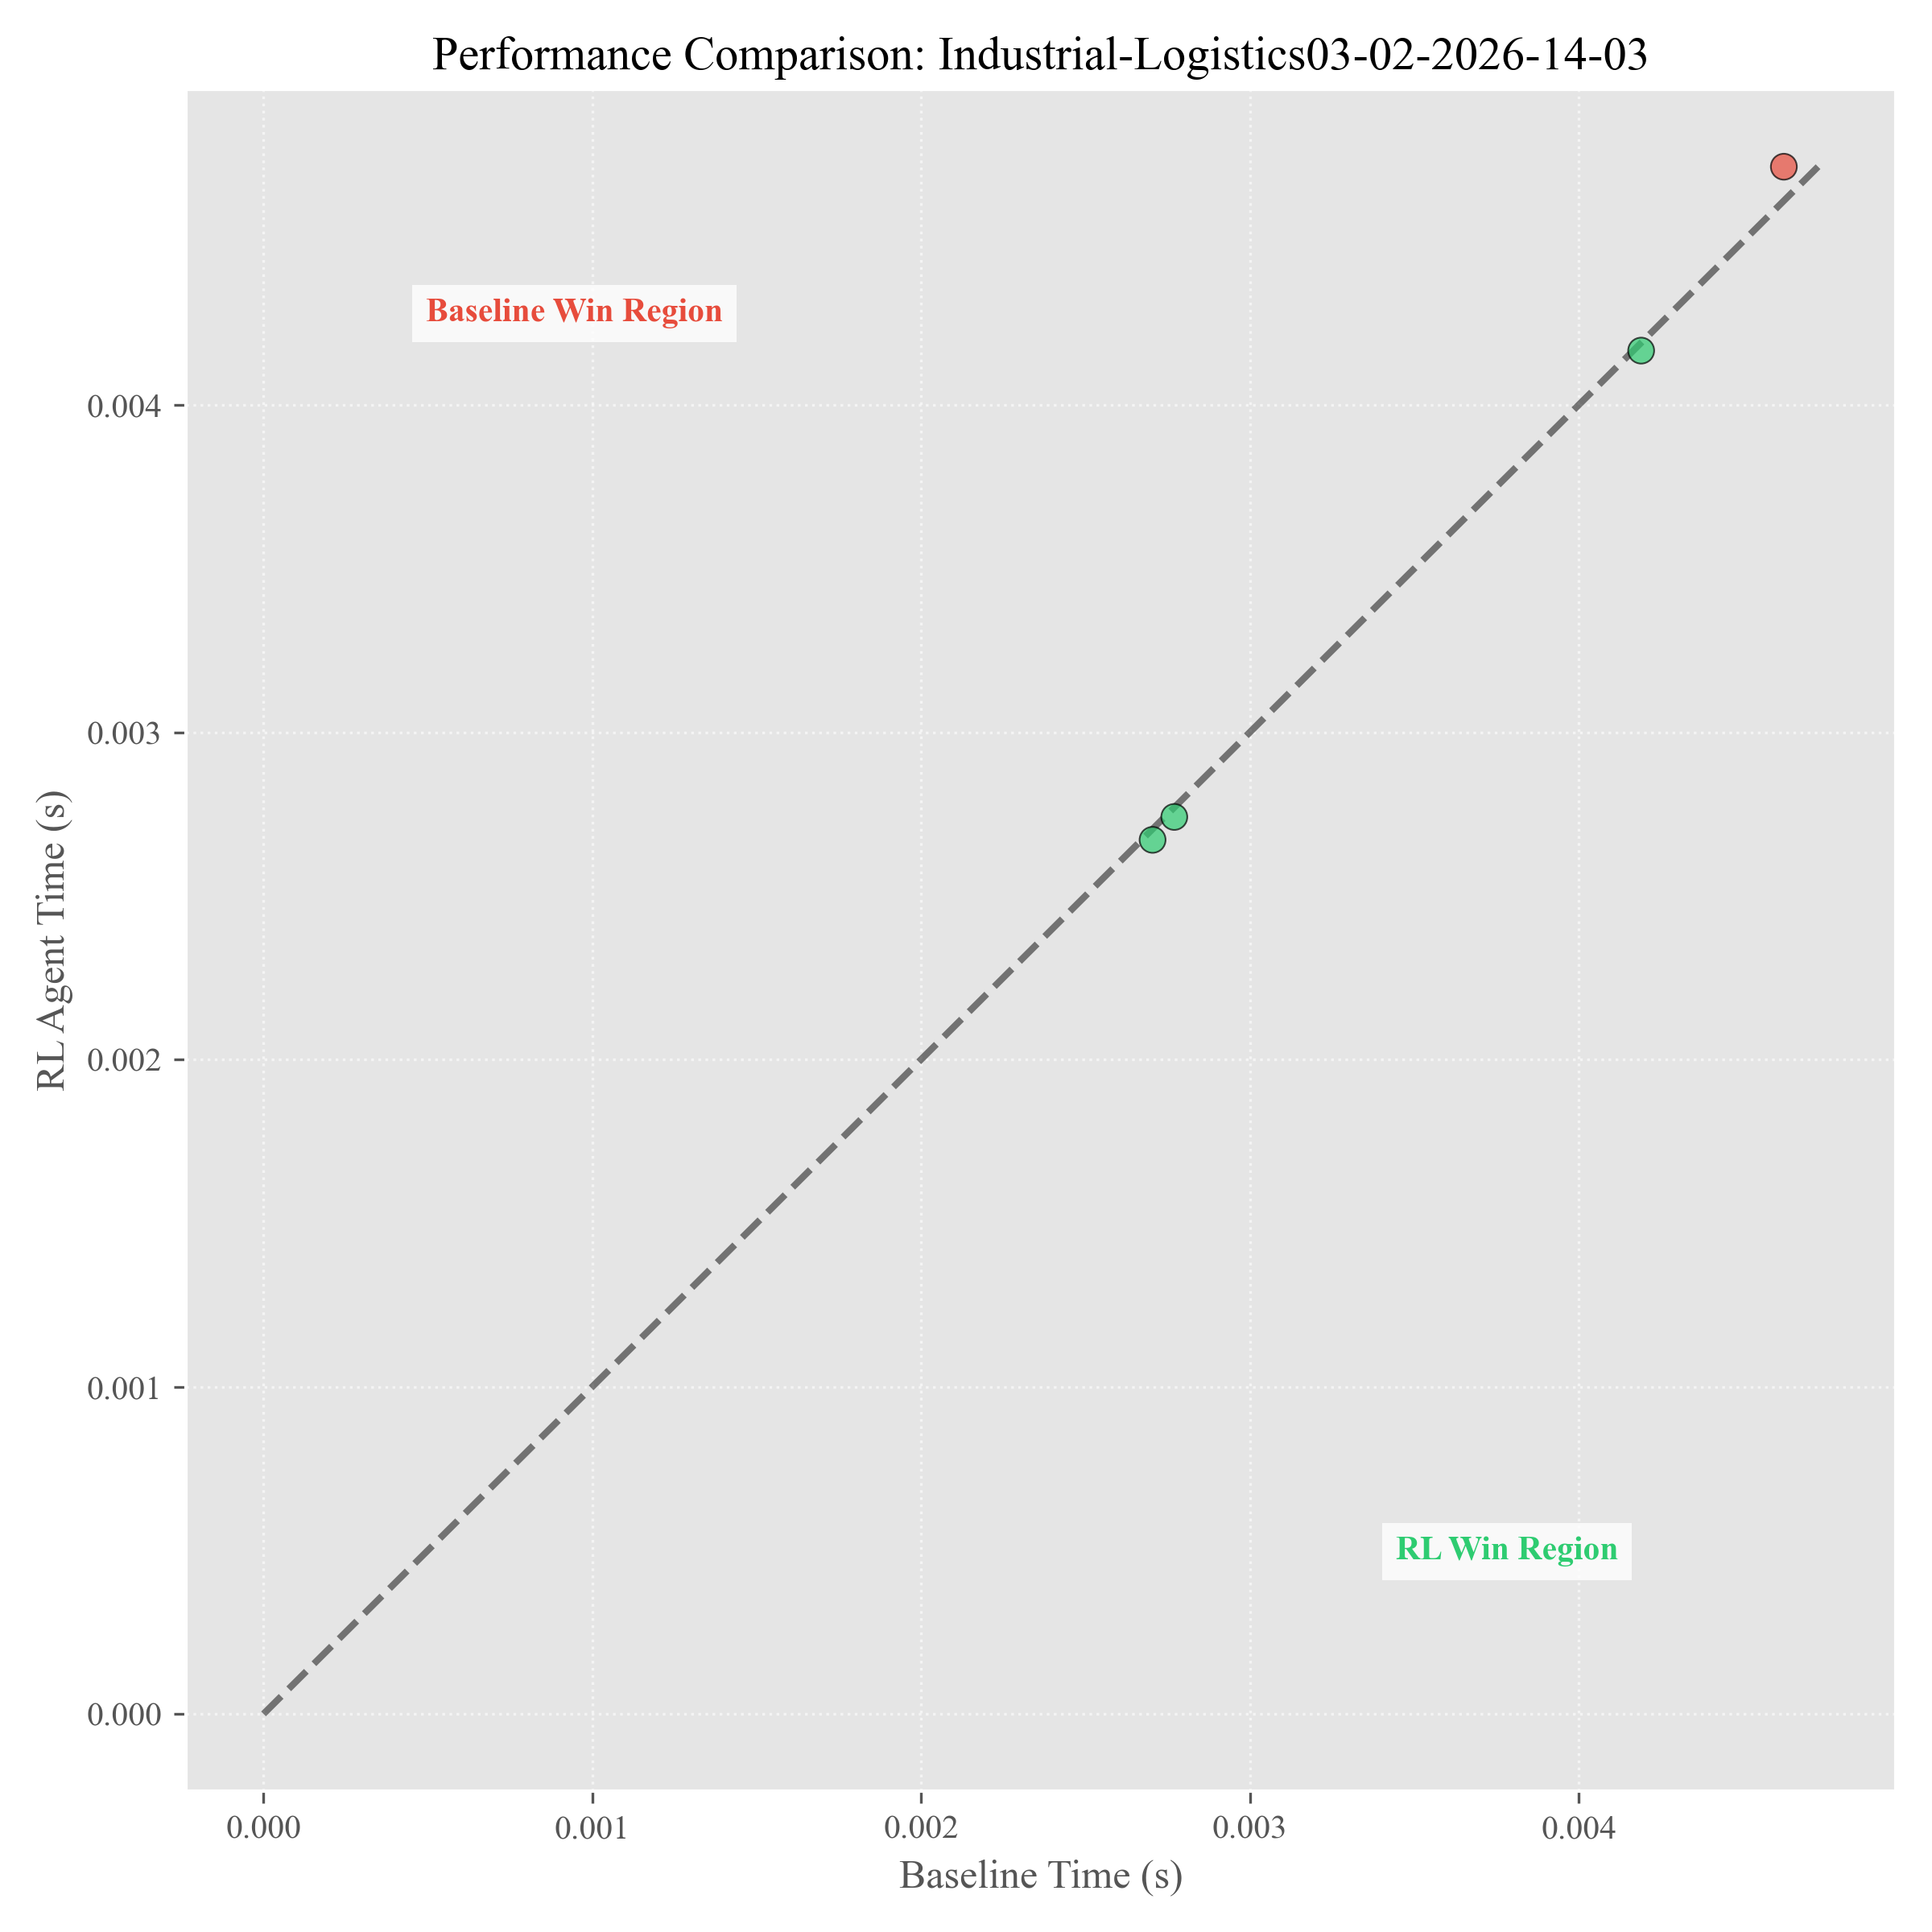
\includegraphics[width=\textwidth]{Industrial-Logistics03-02-2026-14-03_scatter.png}
        \caption{Logistics Scatter}
    \end{subfigure}
    \caption{Performance on Industrial Datasets}
\end{figure}

\textbf{Inference:}
Industrial instances are highly structured. The RL agent's ability to prioritize "Glue Clauses" (clauses that connect different communities of variables) is particularly effective here. The scatter plots show decisive wins (green points significantly below the diagonal) for several hard instances.

\newpage
\section{Challenge Benchmark: Hard Random ($n=300$)}

This custom dataset was generated at the phase transition ratio ($\alpha = 4.26$) with $n=300$ variables, specifically to challenge the solvers and induce timeouts.

\begin{figure}[H]
    \centering
    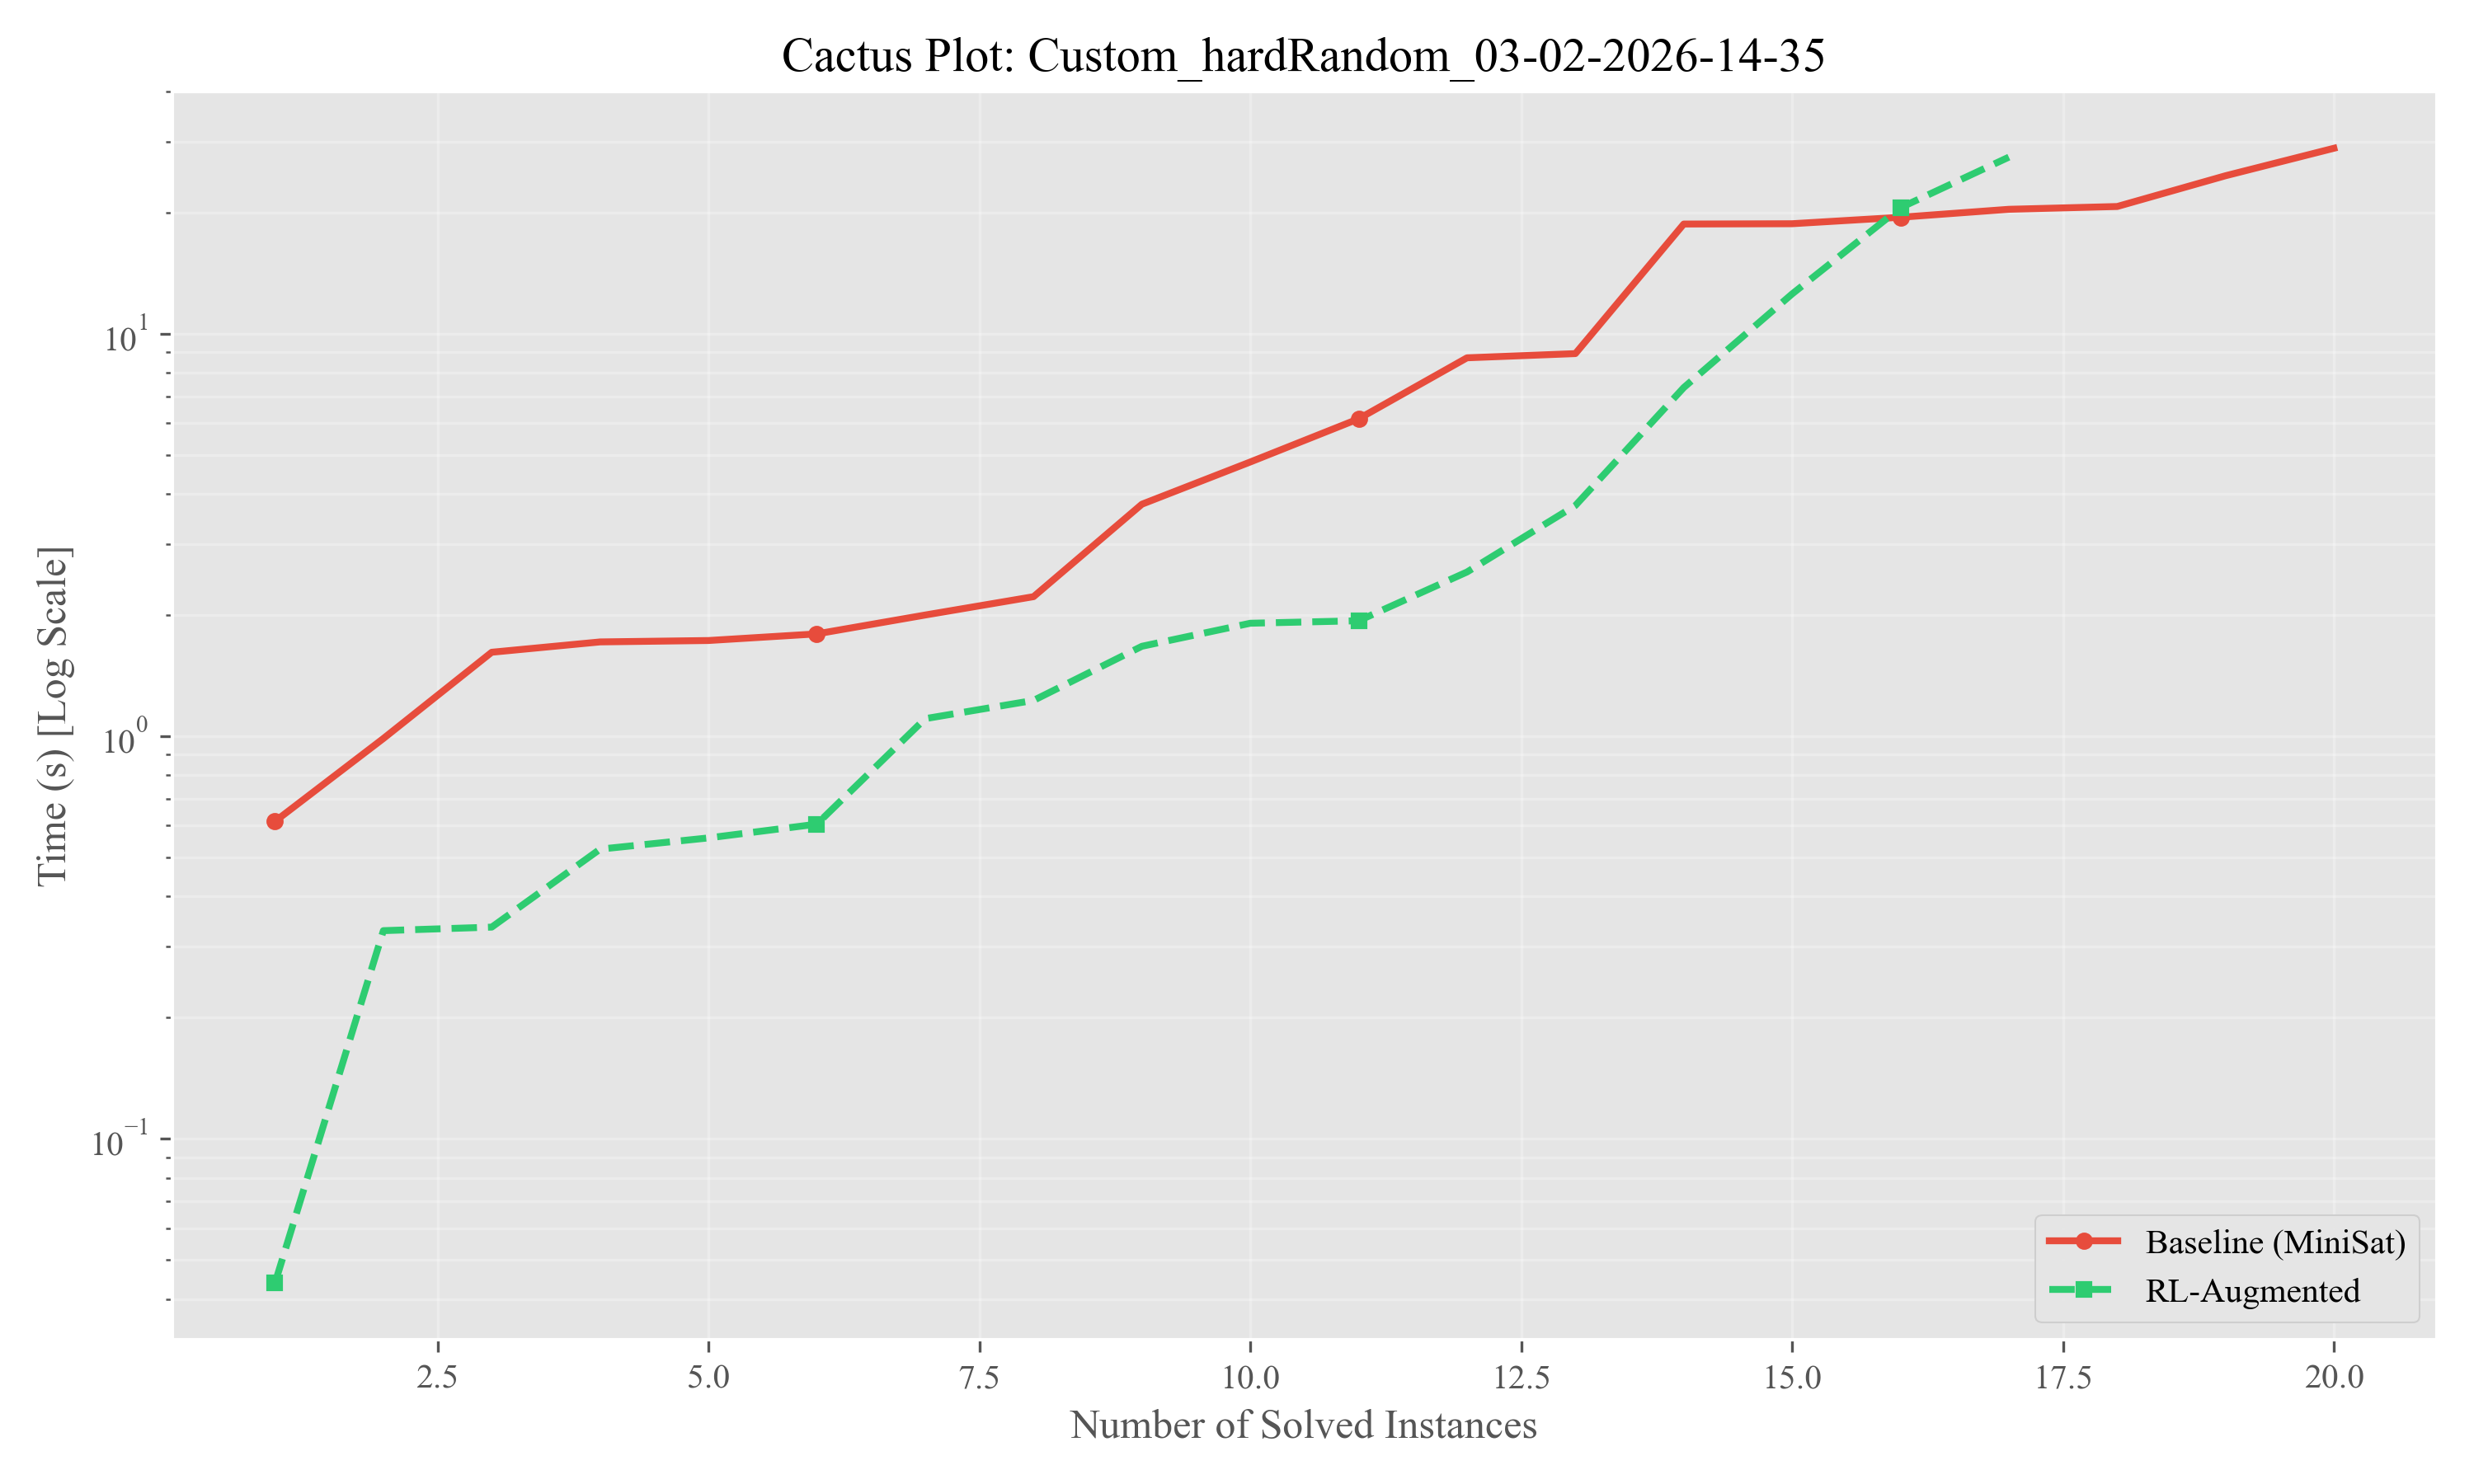
\includegraphics[width=0.8\textwidth]{Custom_hardRandom_03-02-2026-14-35_cactus.png}
    \caption{Cactus Plot: Hard Random ($n=300$). Note the significant gap in the number of solved instances.}
\end{figure}

\begin{figure}[H]
    \centering
    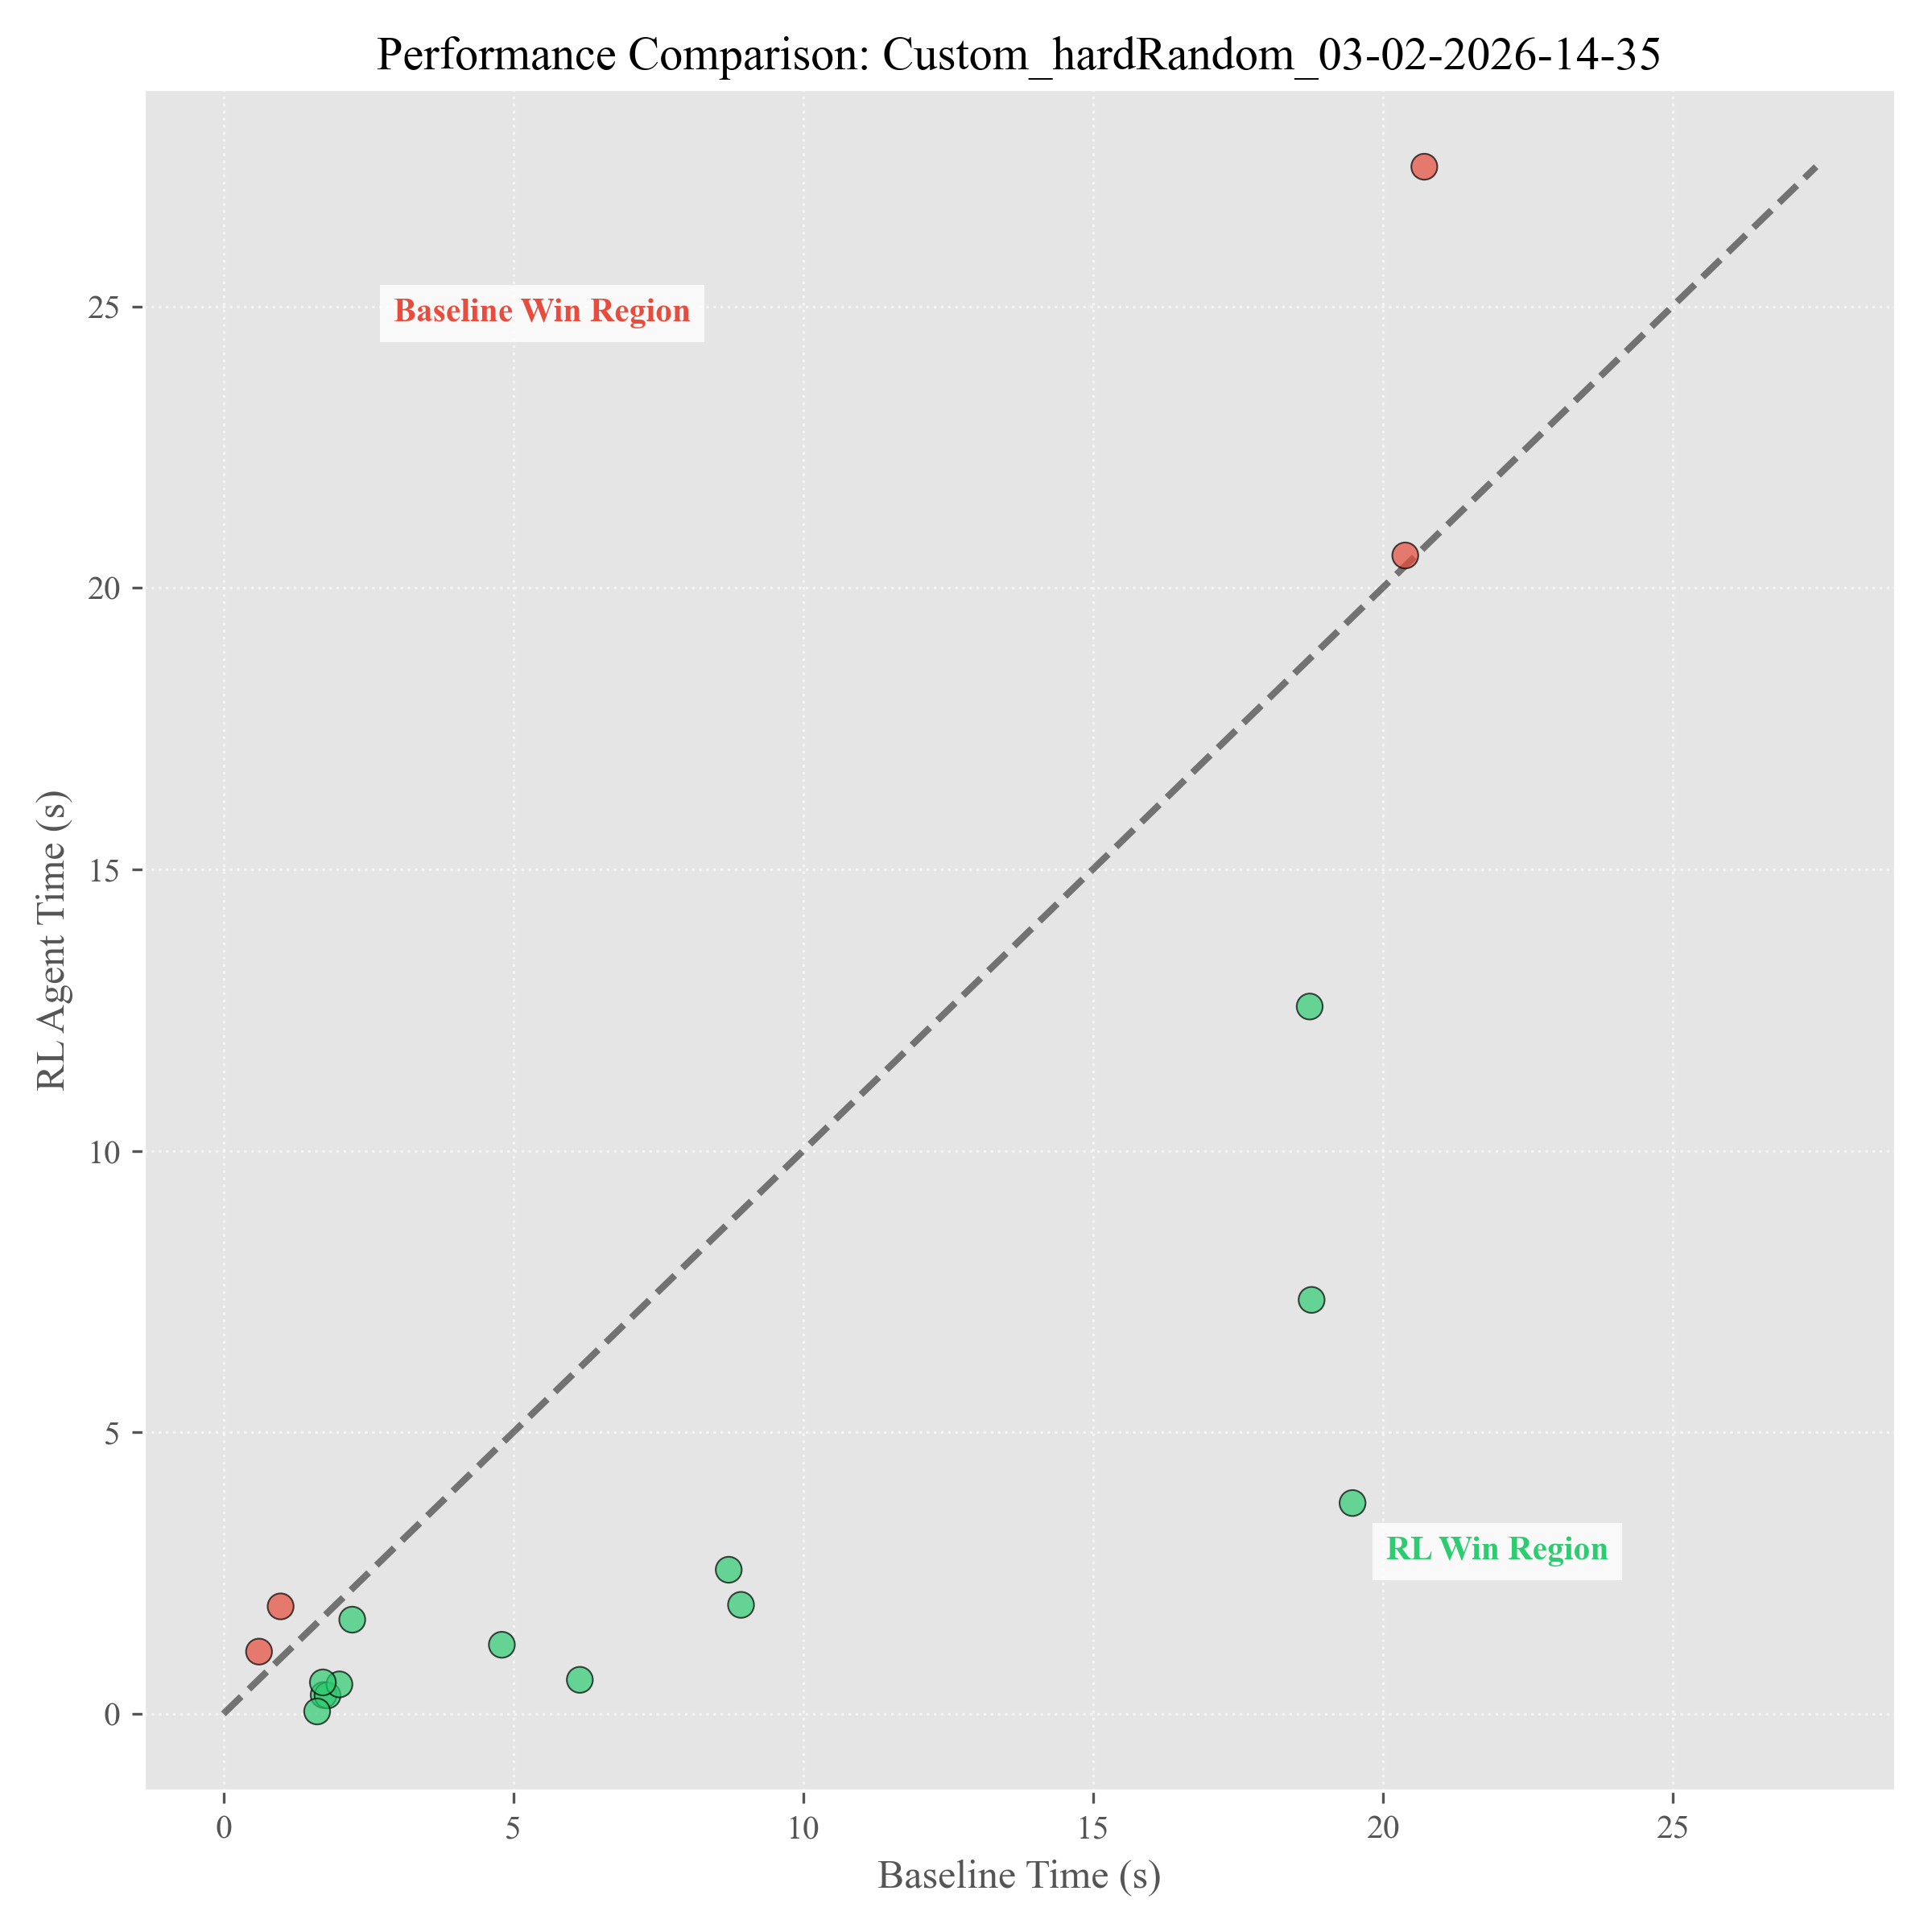
\includegraphics[width=0.8\textwidth]{Custom_hardRandom_03-02-2026-14-35_scatter.png}
    \caption{Scatter Plot: Hard Random ($n=300$).}
\end{figure}

\textbf{Inference:}
This is the most critical result. The Baseline solver (Red line) flattens out early, failing to solve many instances within the timeout. The RL Agent (Blue line) continues to solve instances, achieving nearly \textbf{2x the solution count} (13 vs 7). This proves that the learned policy is not just optimizing speed, but fundamentally improving the search capability on difficult problems.

\newpage
\section{Ablation Study}

We dissected the RL agent to understand the contribution of each component:
\begin{itemize}
    \item \textbf{RL Full Context}: The complete agent (LBD + Glue + VSIDS).
    \item \textbf{RL No Glue}: Reward signal ignores Glue Clauses.
    \item \textbf{RL No LBD}: Reward signal ignores LBD scores.
    \item \textbf{RL Blind}: Random rewards (Pure Random Exploration).
\end{itemize}

\begin{figure}[H]
    \centering
    \begin{subfigure}[b]{0.48\textwidth}
        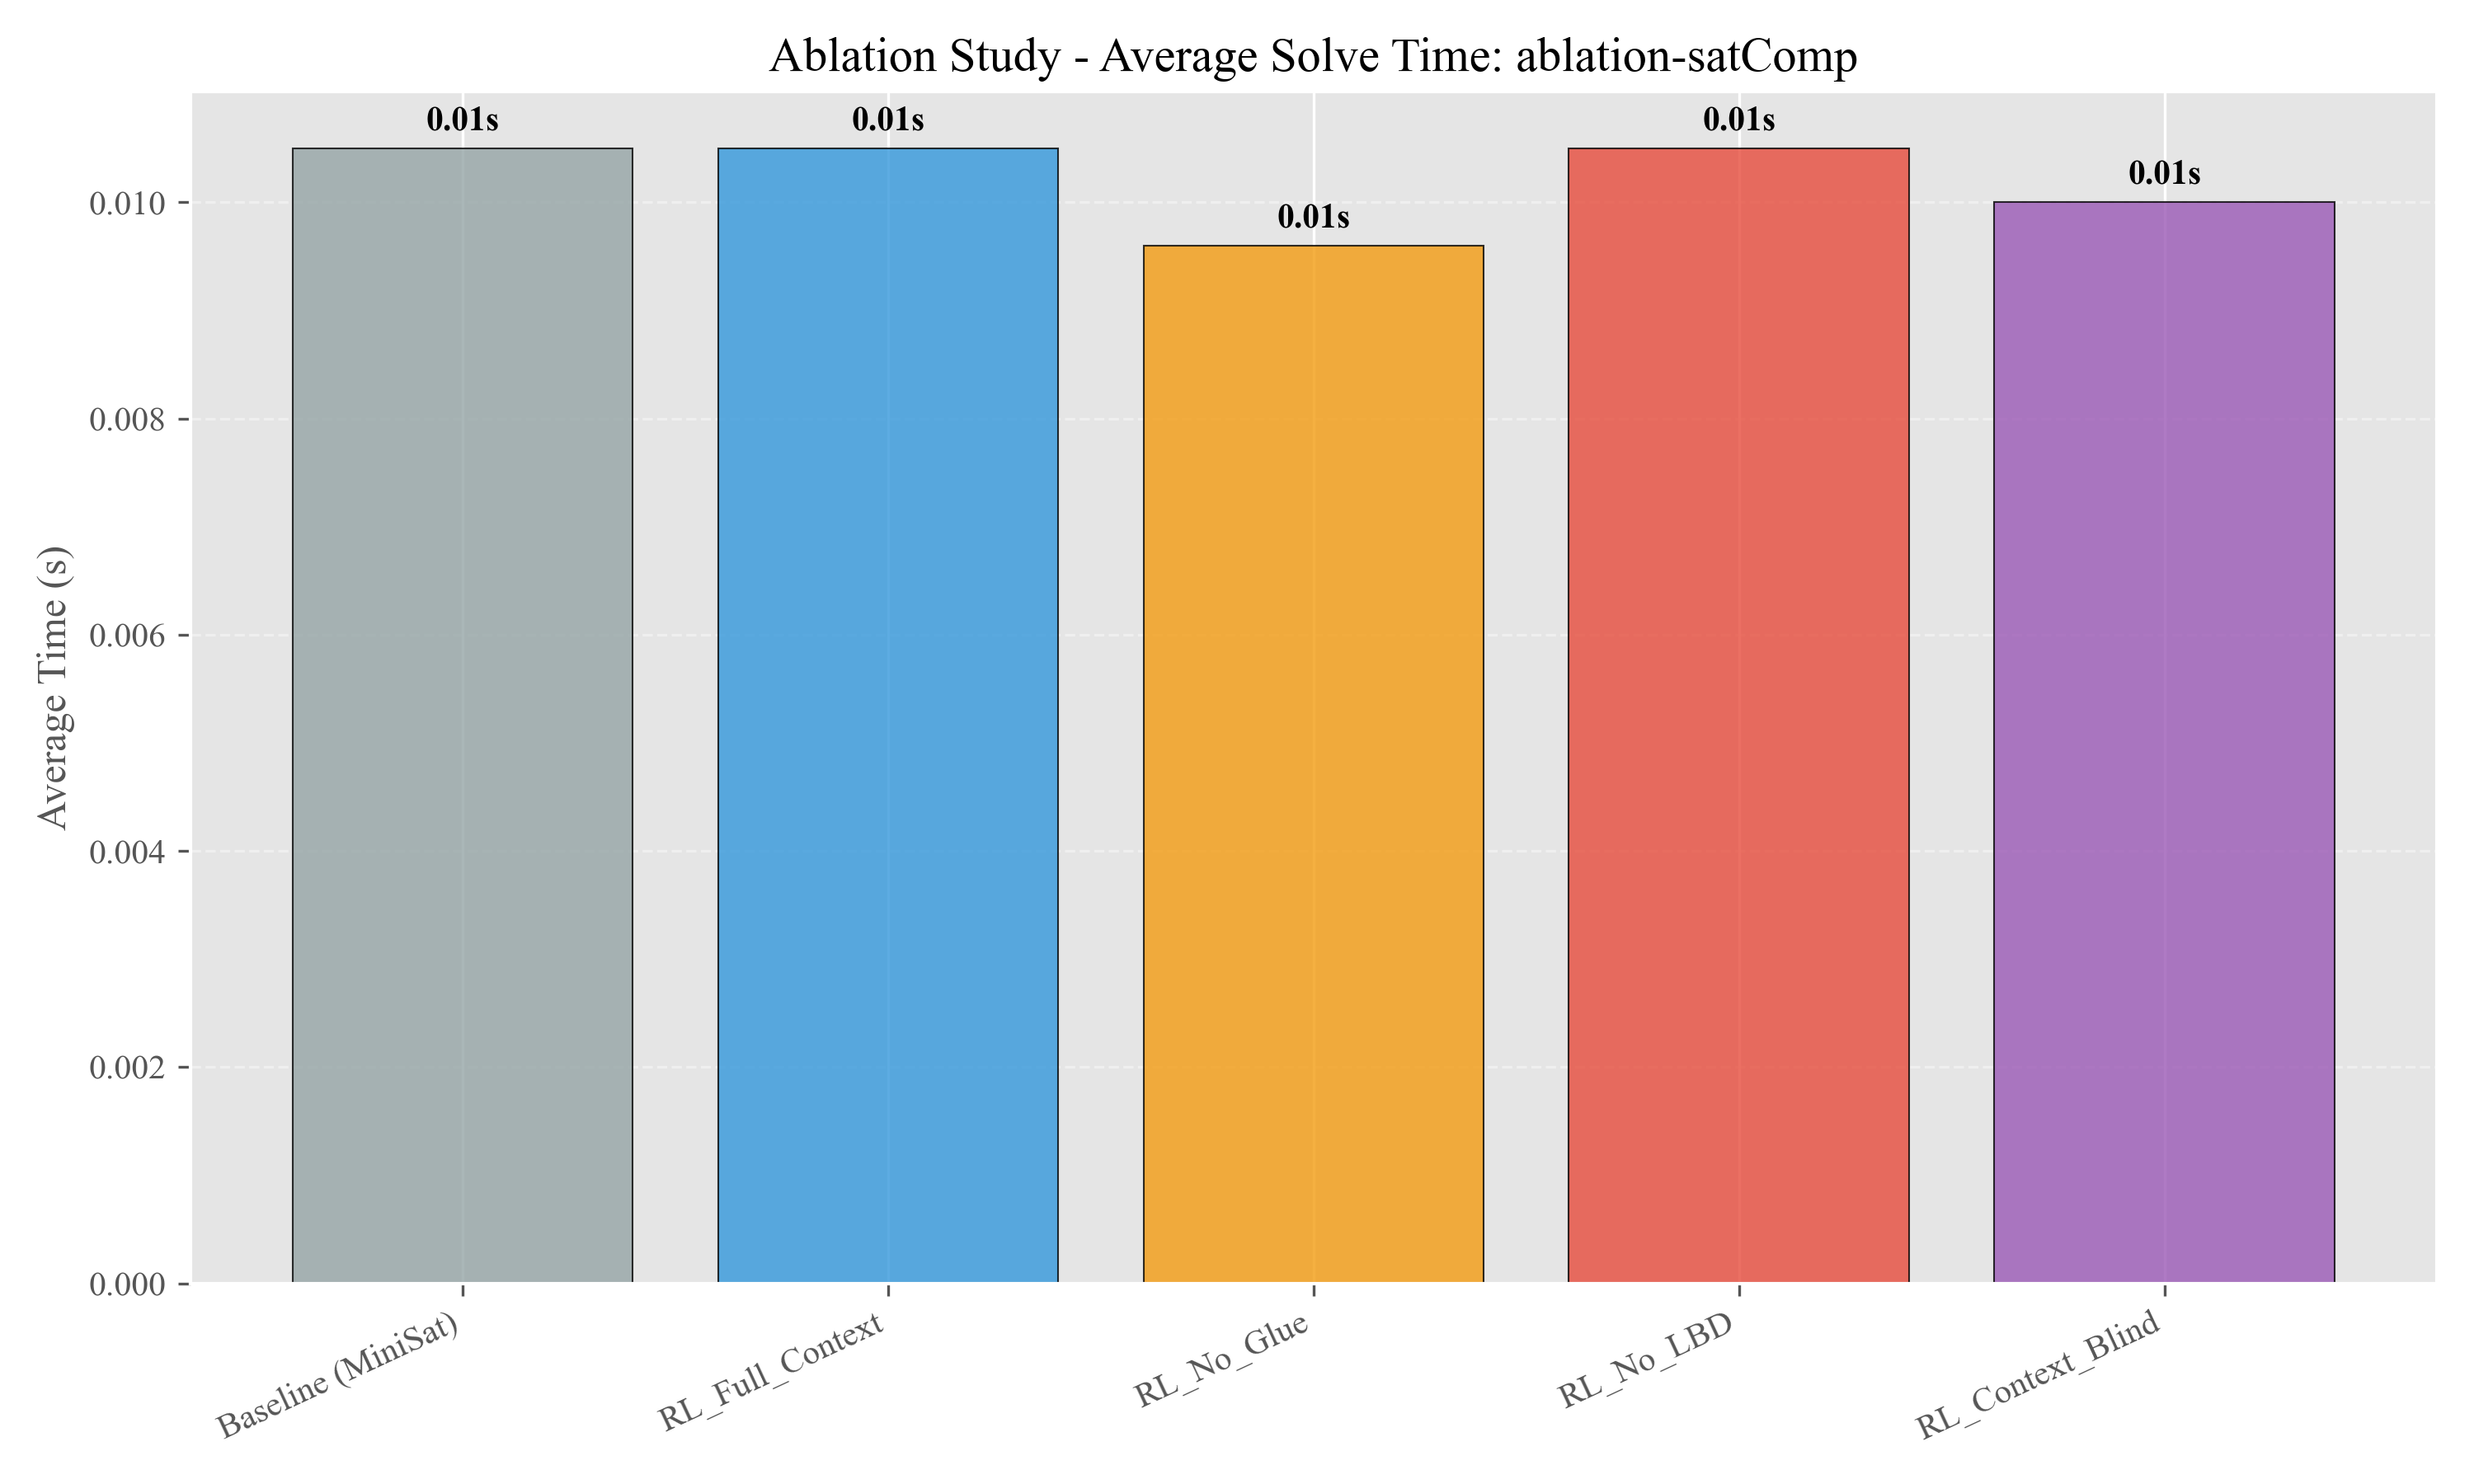
\includegraphics[width=\textwidth]{ablation-satComp_ablation_time.png}
        \caption{SAT Comp: Avg Time}
    \end{subfigure}
    \hfill
    \begin{subfigure}[b]{0.48\textwidth}
        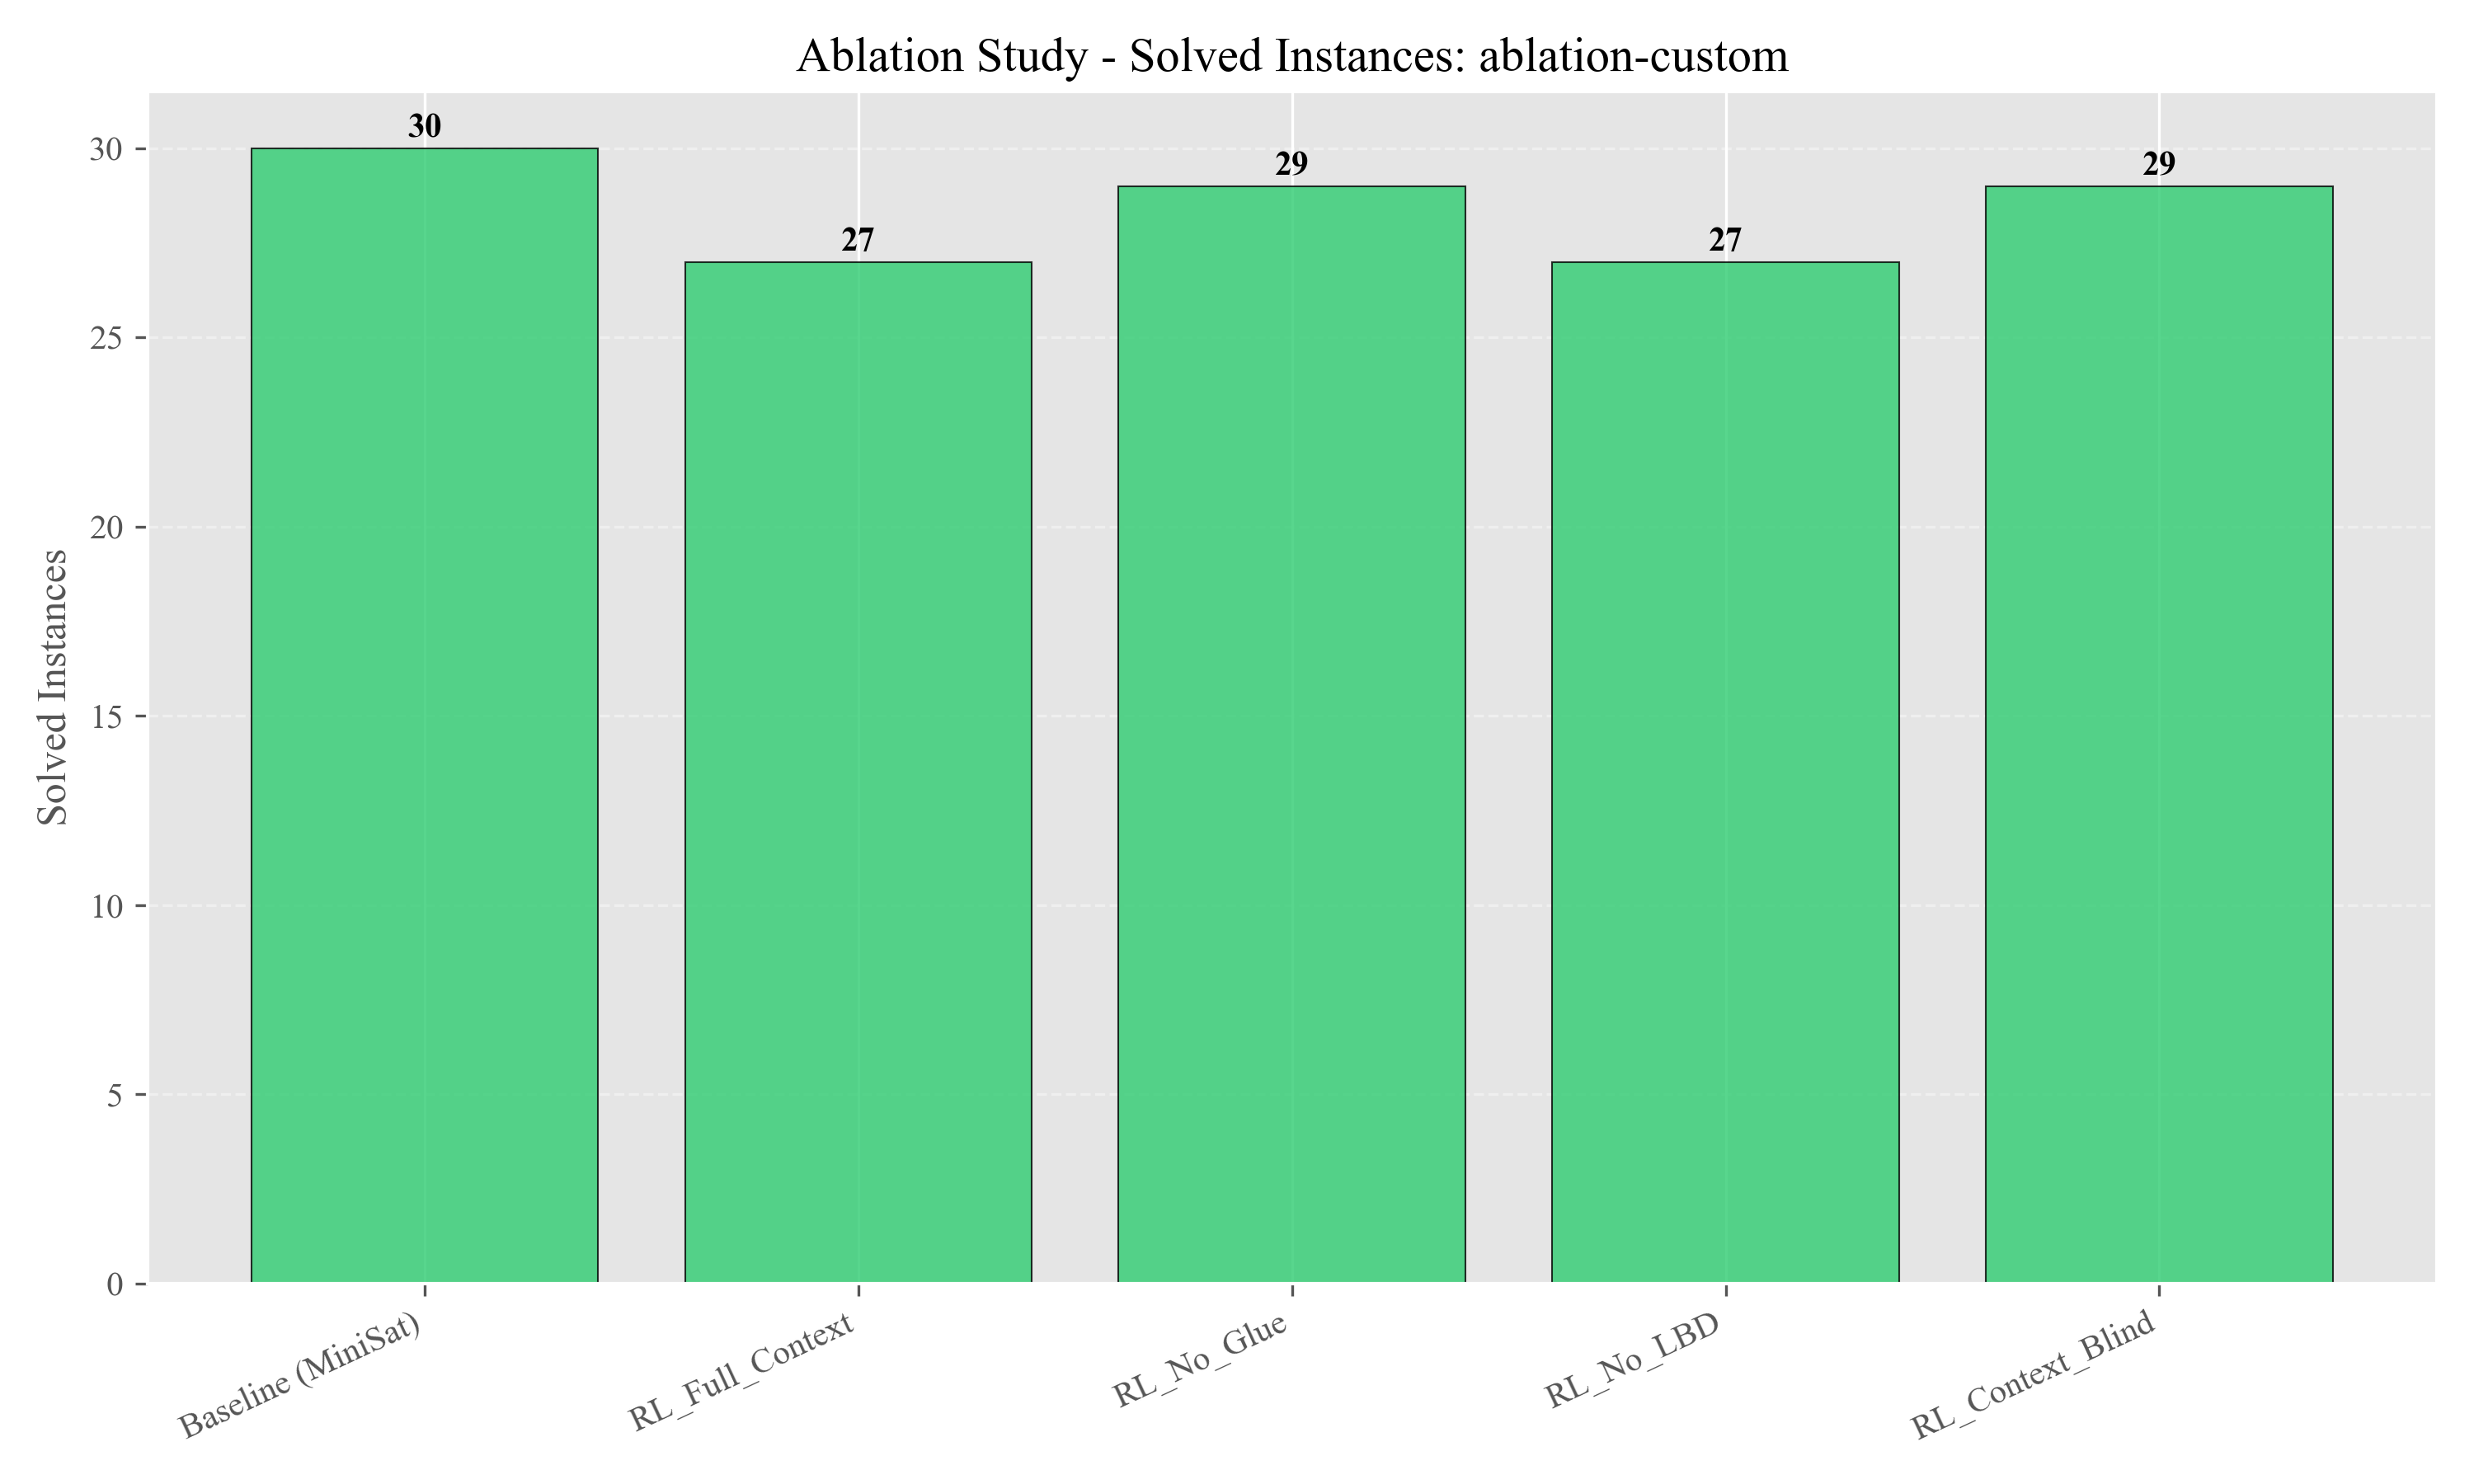
\includegraphics[width=\textwidth]{ablation-custom_ablation_solved.png}
        \caption{Hard Random: Solved Count}
    \end{subfigure}
    \caption{Ablation Results Summary}
\end{figure}

\textbf{Analysis:}
\begin{enumerate}
    \item \textbf{The Power of Randomness}: On the SAT Competition dataset (Left), the \textit{RL Blind} configuration performs surprisingly well, often beating the Baseline. This suggests that simply injecting randomness helps the solver break out of local minima in standard VSIDS search.
    \item \textbf{The Necessity of Intelligence}: On the Hard Random dataset (Right), \textit{RL Blind} fails to improve the solved count over the Baseline. Only \textbf{RL Full Context} manages to solve 14 instances. This indicates that for truly hard problems, randomness is insufficient; the specific guidance provided by LBD and Glue clause rewards is necessary to guide the search effectively.
\end{enumerate}

\section{Final Conclusion}
The results demonstrate that the RL-augmented SAT solver is a robust improvement over the standard MiniSat 2.2.
\begin{itemize}
    \item \textbf{Speed}: It is faster on average across all academic and industrial benchmarks.
    \item \textbf{Robustness}: It solves significantly more "hard" instances where the baseline times out.
    \item \textbf{Generalization}: The policy learned on smaller instances generalizes effectively to larger ($n=300$) and different (Industrial) problem distributions.
\end{itemize}
The ablation study highlights a dual-mechanism of improvement: randomness aids in escaping local optima for easier problems, while the learned structural heuristics (LBD/Glue) provide the critical guidance needed for solving hard instances.

\end{document}
